\documentclass[11pt,letterpaper]{article}
\input{headings}
\newcommand \recipeName {Puffy Pastry}
\newcommand \fileName {PuffPastry}
\chead{\recipeName}

\begin{document}
\input{title}

\begin{flushright}
From {\it  The French Chef} by Julia Child.
\end{flushright}
 
This is the best recipe for Puff Pastry that I ever made. It is not difficult, but you need to read the recipe carefully before starting. The resting times are very important because a successful puff pastry is achieved when the components and the dough are kept cold at all times.

\begin{description}

\item[Ingredients:]\ \\
	\begin{itemize}
	\item 2 3/4 cups unbleached all-purpose flour (13 1/2 oz)
	\item 3/4 cups cake flour (3 oz)
	\item 2 teaspoons salt 
	\item 1/4 cup flavourless cooking oil (1 3/4 oz)
	\item 1 cup ice water (8 oz)
	\item 3 sticks cold unsalted butter (12 oz)
	\end{itemize}

\item[Procedure:]\ \\
	\begin{enumerate}
	\item {\bf Mix the Dough}
	\begin{itemize}
	\item Mix the flours with a rubber spatula.
	\item Remove 1/2 cup of the mixed flours and reserve for later.
	\item Drizzle the oil over the flour and mix thoroughly with a rubber spatula.
	\item Dissolve the salt in the ice water.
	\item Add water all at once.
	\item Cutting and stirring with the spatula, mix until dough comes together.
	\item Use fingers to press the dough together.
	\item Transfer dough to working surface and press it all together into a ball.
	\item Wrap the dough in waxed paper.
	\item Slip into a plastic back.
	\item Refrigerate for at least 40 minutes.
	\end{itemize}
	
	\item {\bf Prepare the butter}
	\begin{itemize}
	\item Place the three sticks of butter side by side on counter.
	\item Beat the butter with a rolling pin until it is about 3/4 inch thick. 
	\item Sprinkle the reserved 1/2 cup of mixed flours on top of the butter.
	\item Using the heel, not the palm, of your hand, press the butter into the working surface to incorporate the flour into the butter.
	\item Using the bench scrapper form the butter into a 15 x 12 inches rectangle.
	\item Open a piece of waxed paper into the counter.
	\item Using bench scrapper lift the butter rectangle into the waxed paper.
	\item Put in the refrigerator for at least 20 minutes.
	\end{itemize}
	\item {\bf Add butter to dough}
	\begin{itemize}
	\item Lightly flour your work surface.
	\item Open the chilled dough pressing with your hands.
	\item Roll it to form a 16 x 18 inches rectangle. So that the 16 inch side is towards you.
	\item Place the butter rectangle to one end of the dough rectangle farther from you so that the butter covers 2/3 of the dough rectangle. Leave 1/2 inch around the butter rectangle uncovered. The 1/3 of the dough rectangle that is not covered by the butter is closer to you and is called the flap.
	\item Fold the flap over the butter so that half of the butter is covered by it.
	\item Fold the resulting rectangle in half so that now all the butter is covered by dough.
	\item Gently press with your fingertips all around to seal the butter within the dough.
	\item Rotate the dough a quarter turn so that the shorter side is in front of you. 
	\end{itemize}
	\item {\bf Make the four-layer fold}
	\begin{itemize}
	\item Press with the rolling pin at intervals equal to the width of your rolling pin starting in the end close to you making small indentations in the dough all the way to the other end.
	\item Roll the dough to a 16 x 8 inches rectangle.
	\item If there are breaks in the dough that expose the butter, sprinkle them with a bit of flour.
	\item Fold both long ends of the rectangle to the center so that the two edges meet at the center.
	\item Fold again in half so that those edges are no longer visible.
	\item Press with two fingers in the middle of the folded rectangle so that you remember that you have completed the second fold.
	\item Wrap the dough in the waxed paper, slip in a plastic bag, and put in the refrigerator for at least 40 minutes.
	\end{itemize}
	\item {\bf Make turns 3 and 4}
	\begin{itemize}
	\item Unwrap the chilled dough and lightly flour it on both sides.
	\item Make indentations with your rolling pin into the dough. First lengthwise and then crosswise. This will make it easier to roll the chilled dough out. 
	\item Roll the dough to a 16 x 18 inches rectangle. 
	\item Fold this rectangle into three just like you fold a business letter.
	\item Rotate the dough a quarter turn so the the shorter side of the folded rectangle is in front of you.
	\item Roll the dough again into a 16 x 18 inches rectangle.
	\item Fold again like a business letter.
	\item Make four indentations on top.
	\item Wrap in the wax paper, slip into a plastic bag and put in the refrigerator.
	\item This dough has 72 layers of butter and is ready to use as is. It needs to refrigerate for two hours before using. It will last in the refrigerator for up to five days and it can be frozen.
	\end{itemize}
	\item {\bf Make turns 5 and 6 --- for extra puffing}
	\begin{itemize}
	\item After the dough refrigerated for at least 40 minutes, repeat turns 3 and 4 to create 648 layers of butter.
	\item Refrigerate for two hours before using the dough.
	\end{itemize}
	\end{enumerate}
\end{description}

\begin{table}
\begin{tabular}{cccc}
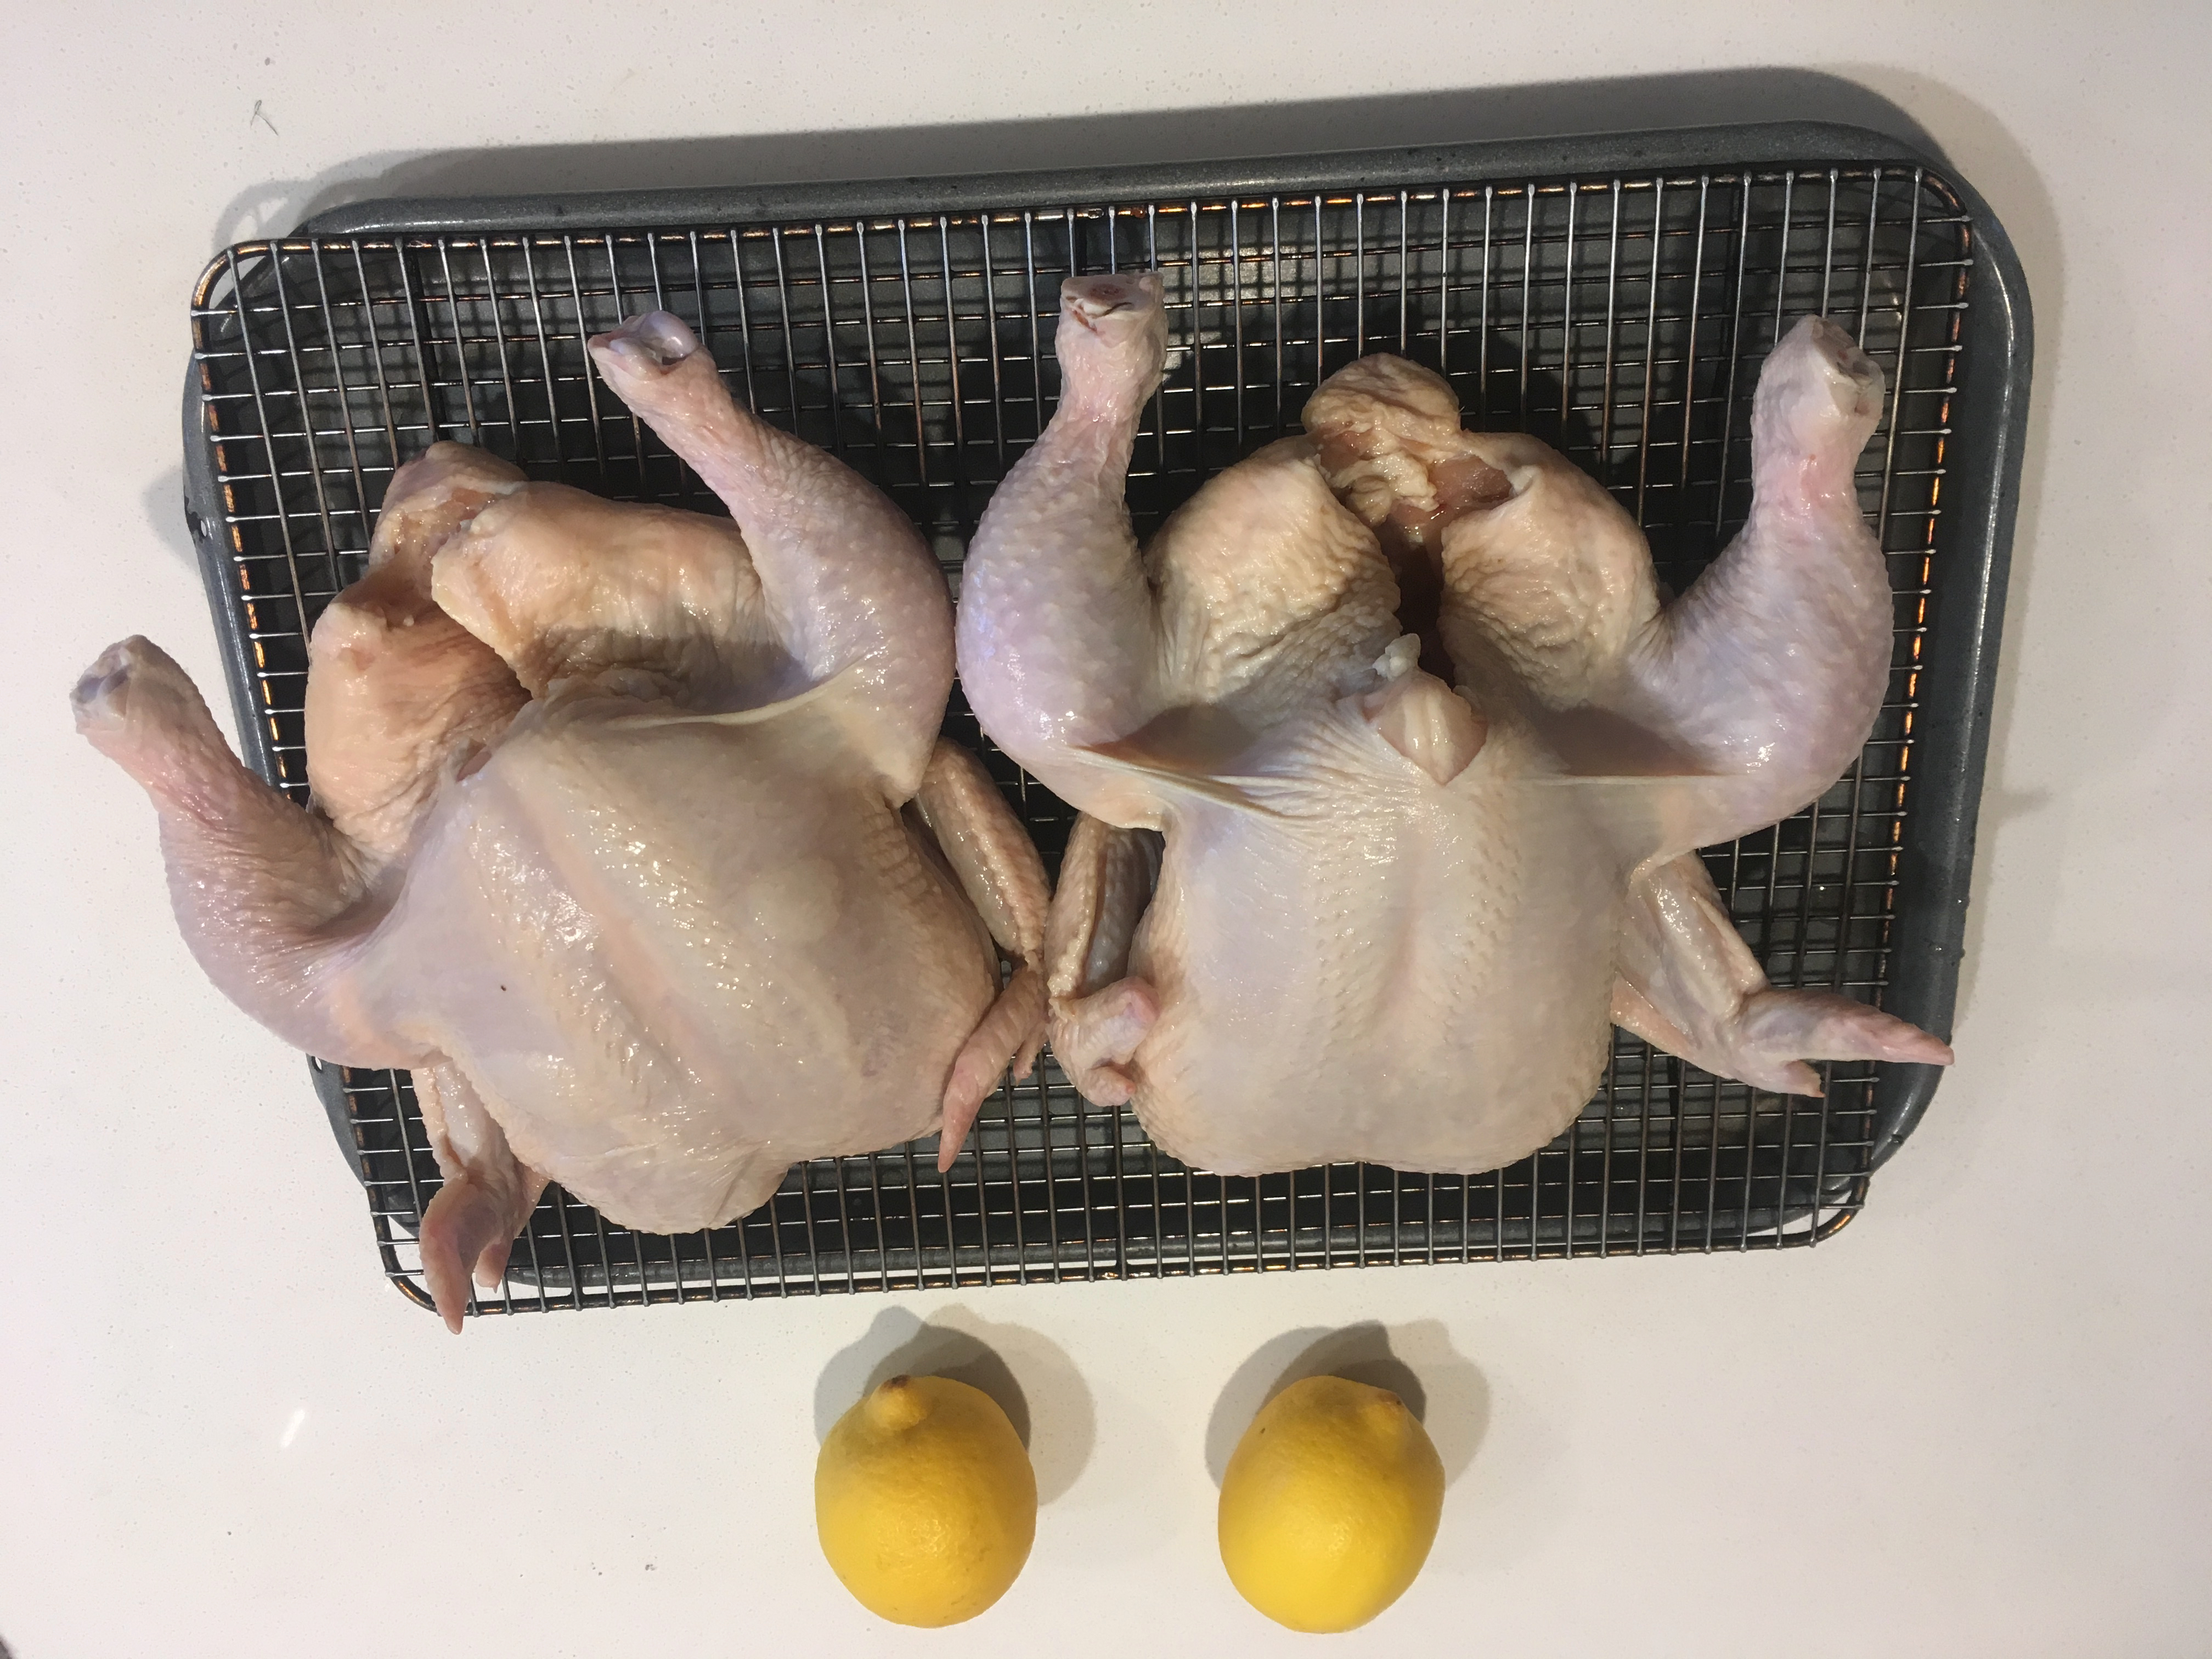
\includegraphics[width=0.25\textwidth]{\imageDir/\fileName/IMG_3197.jpg} &
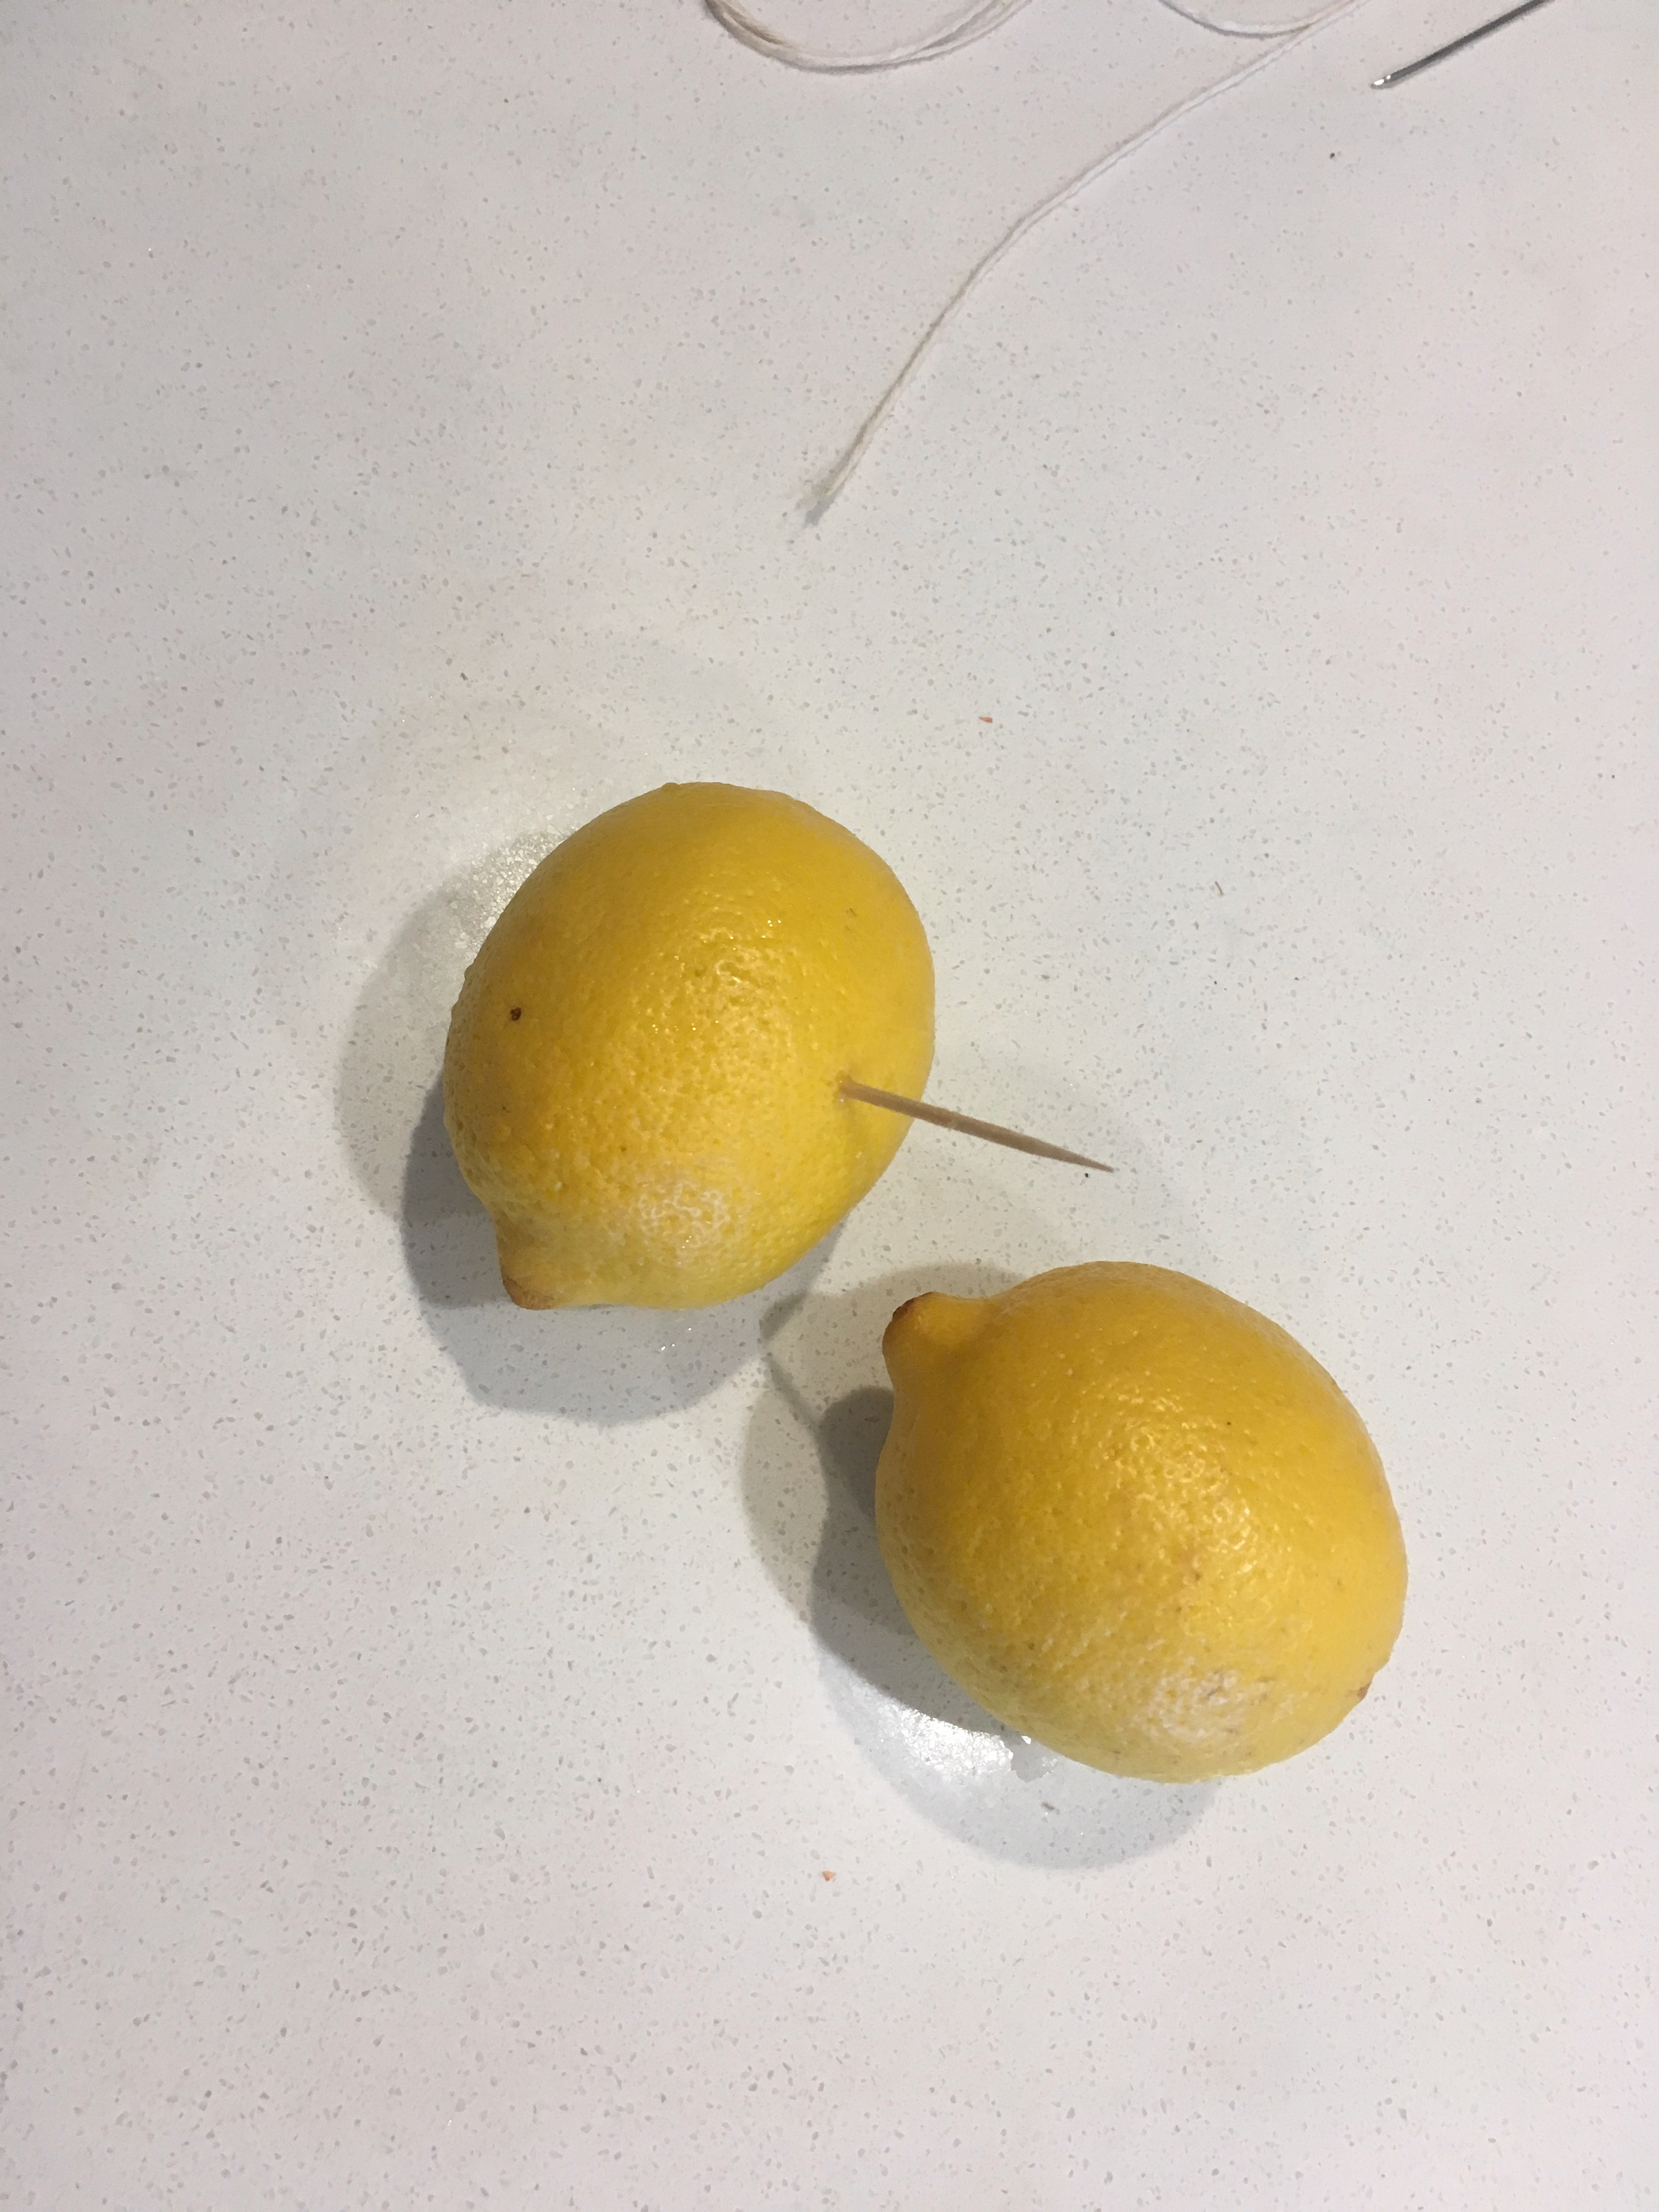
\includegraphics[width=0.25\textwidth]{\imageDir/\fileName/IMG_3212.jpg} &
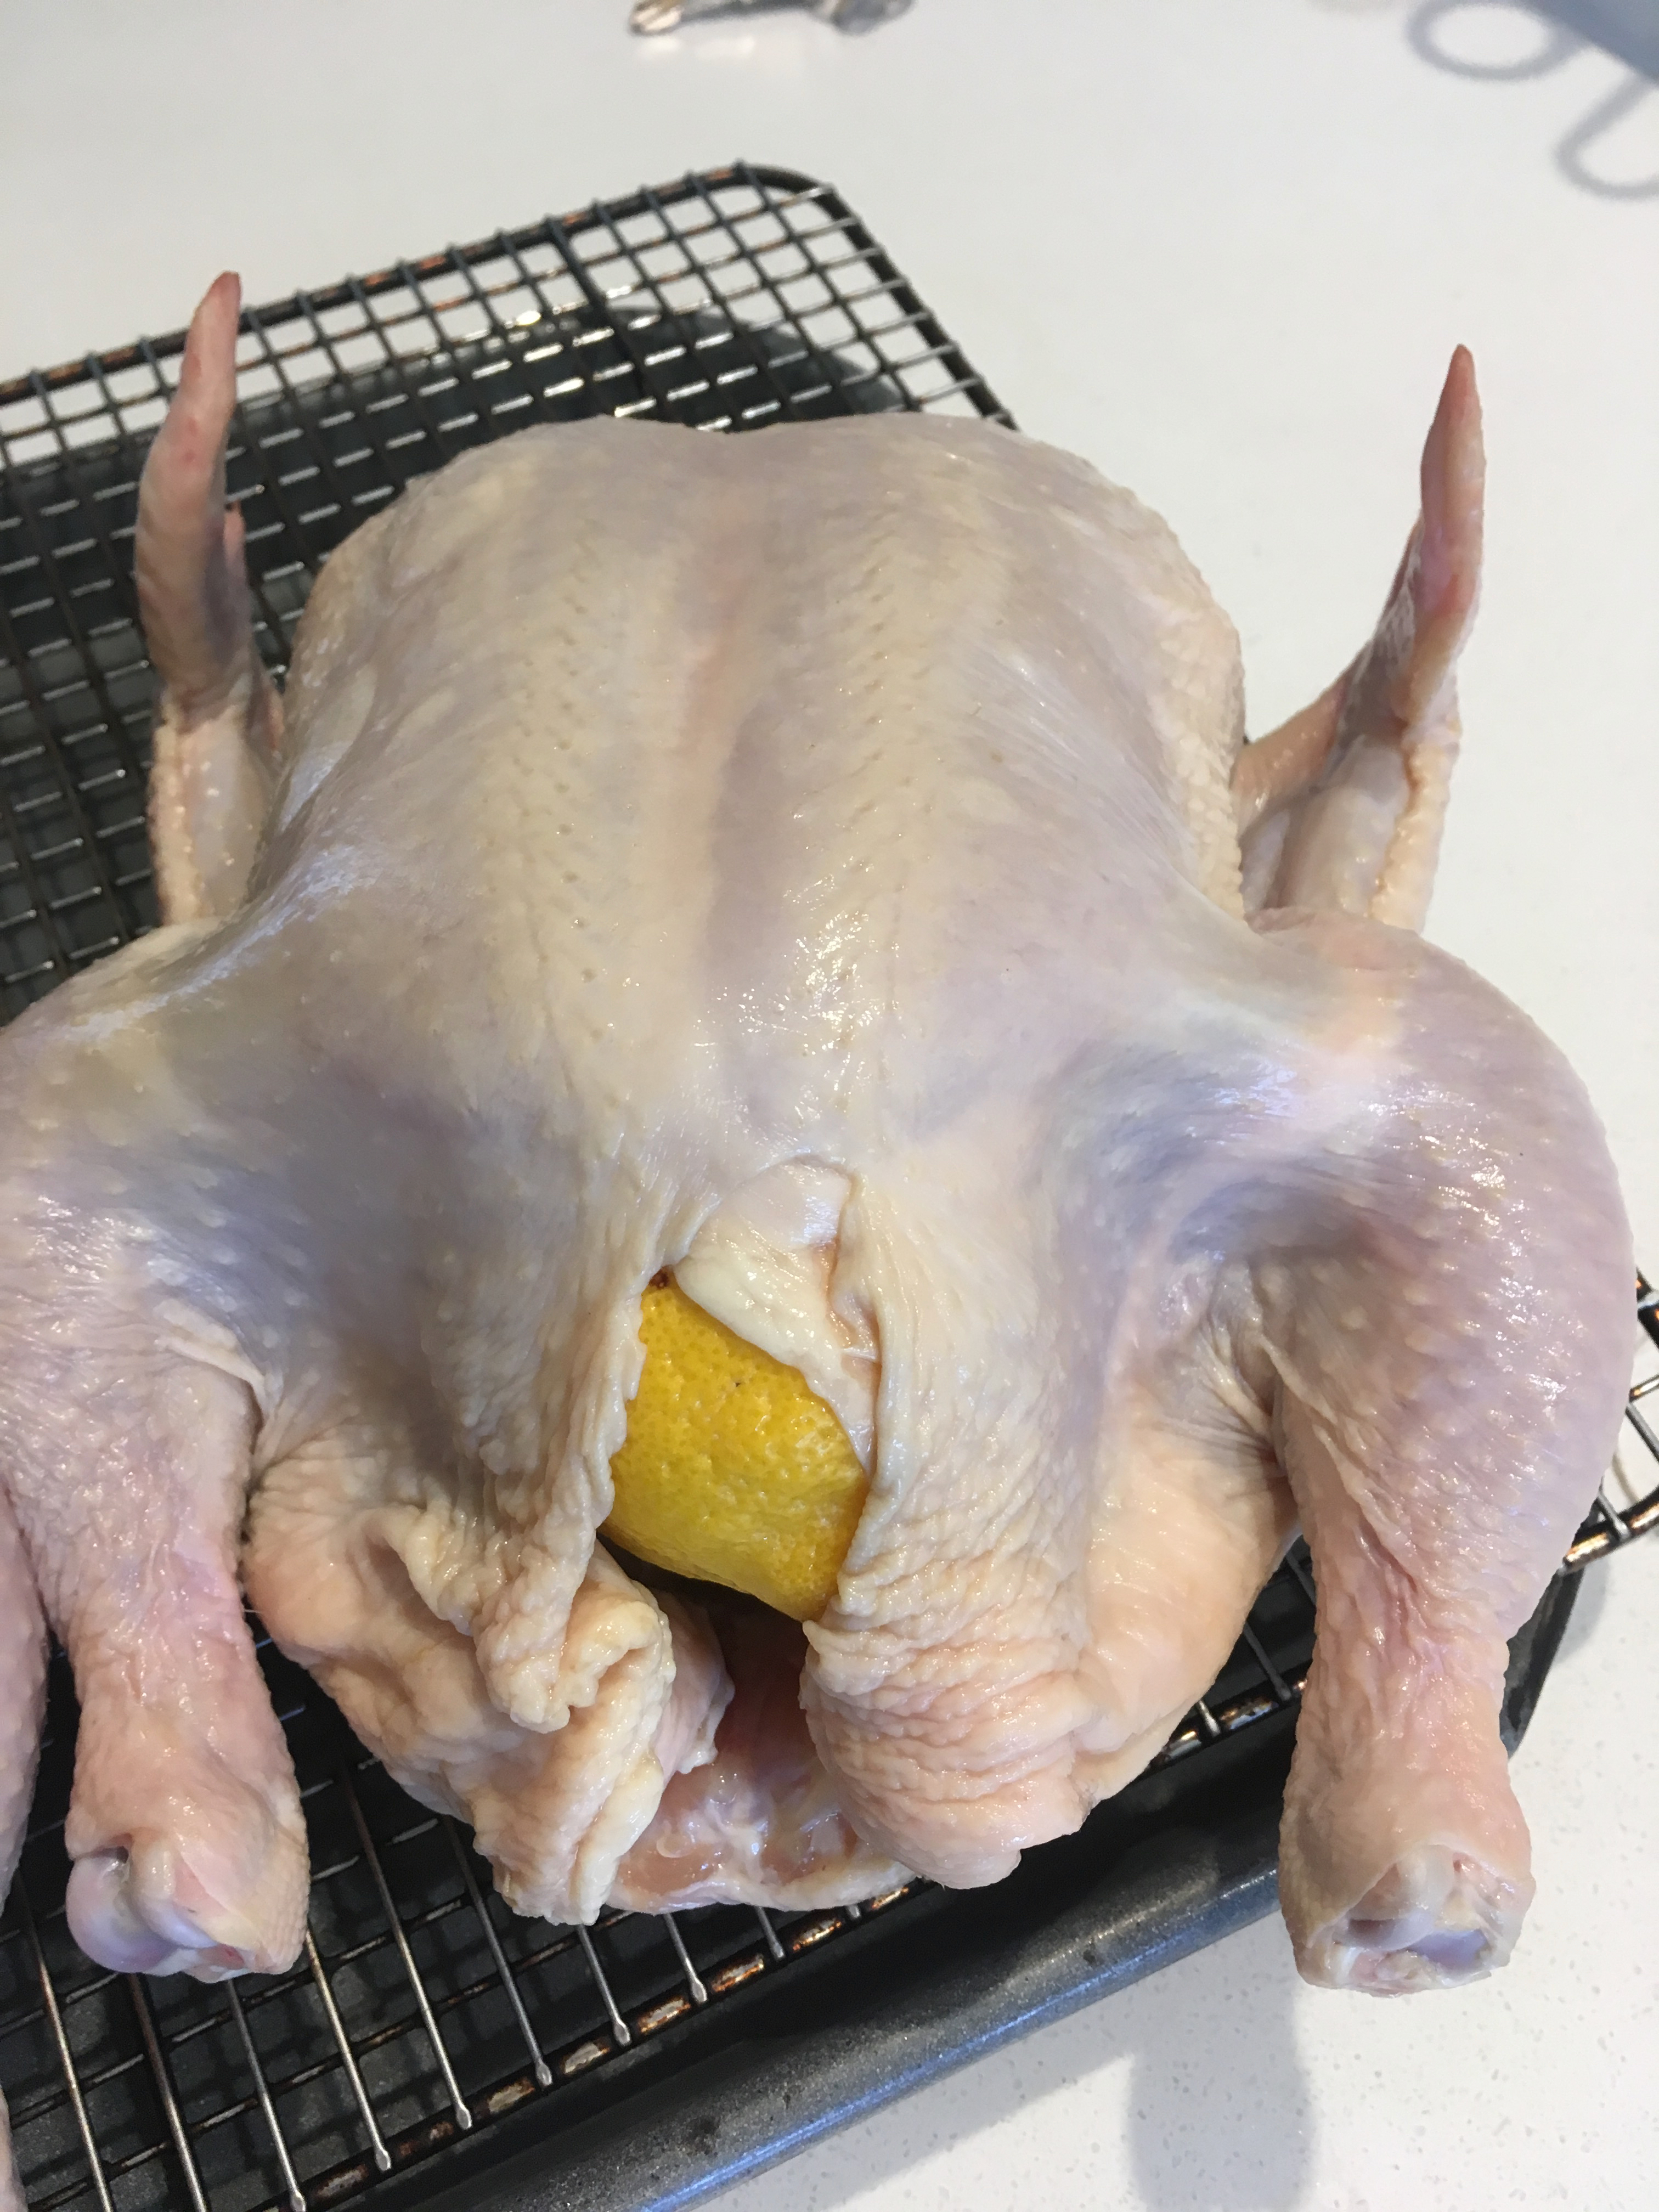
\includegraphics[width=0.25\textwidth]{\imageDir/\fileName/IMG_3213.jpg} \\
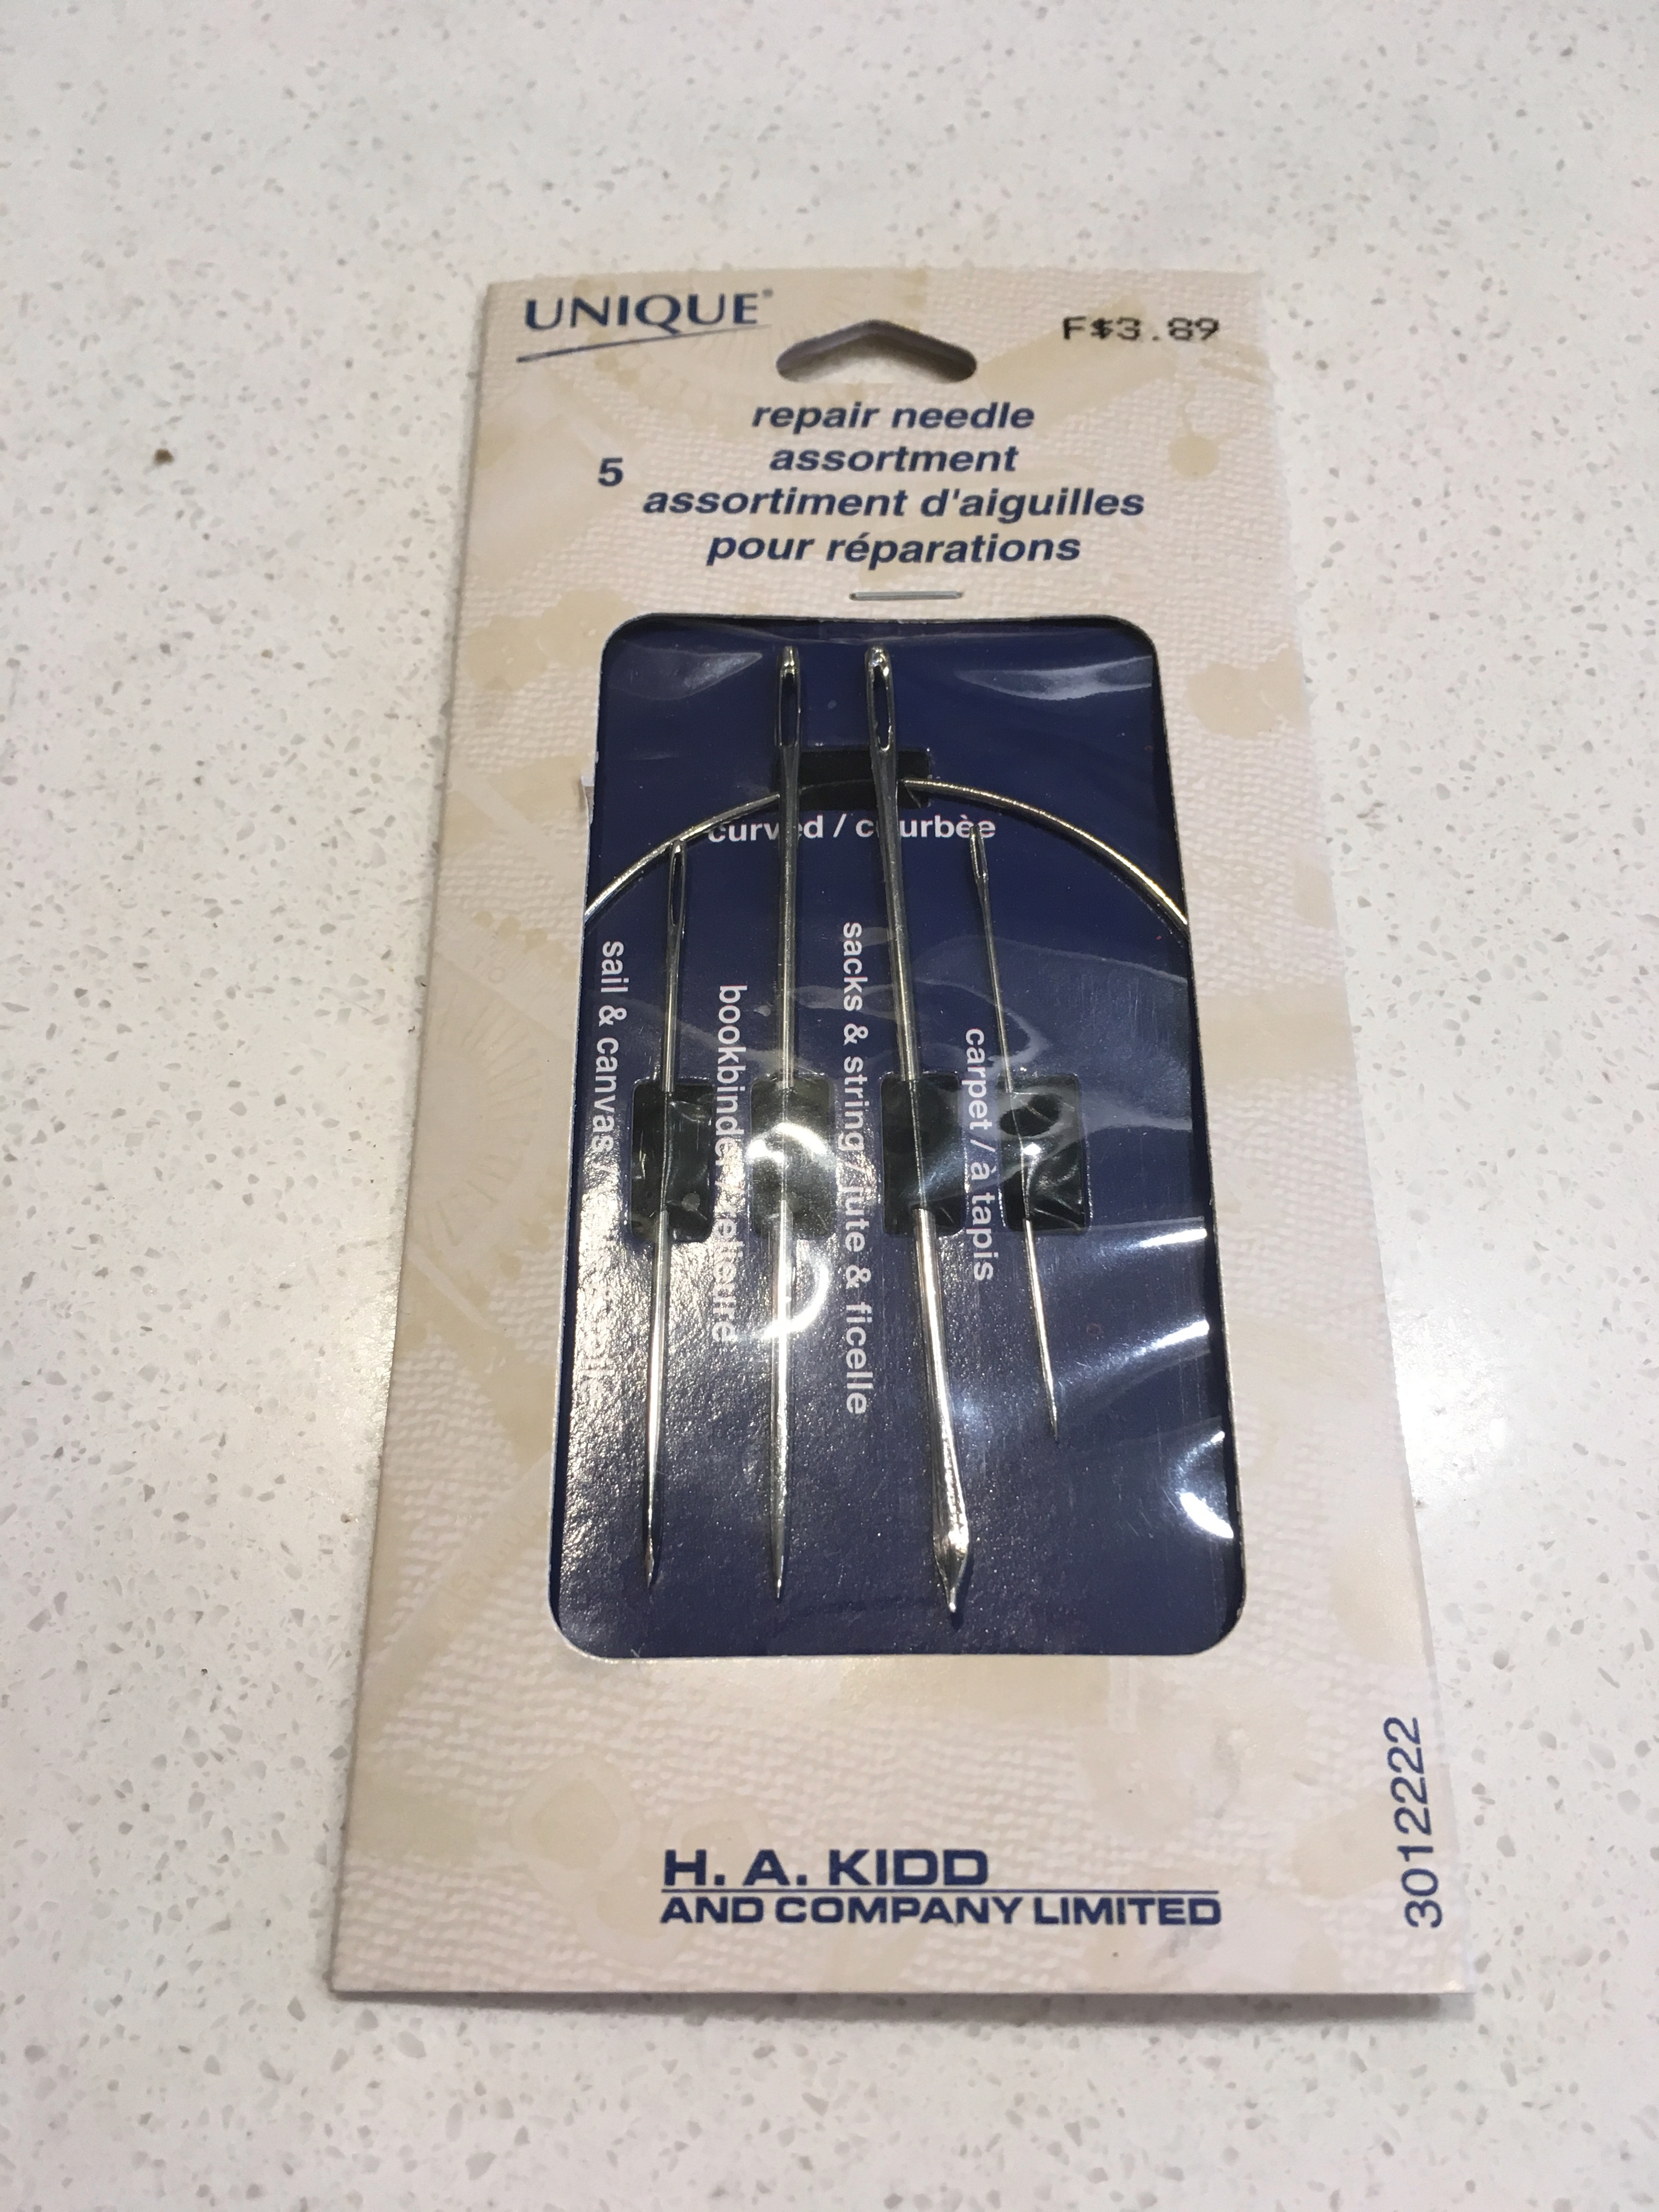
\includegraphics[width=0.25\textwidth]{\imageDir/\fileName/IMG_3206.jpg} &
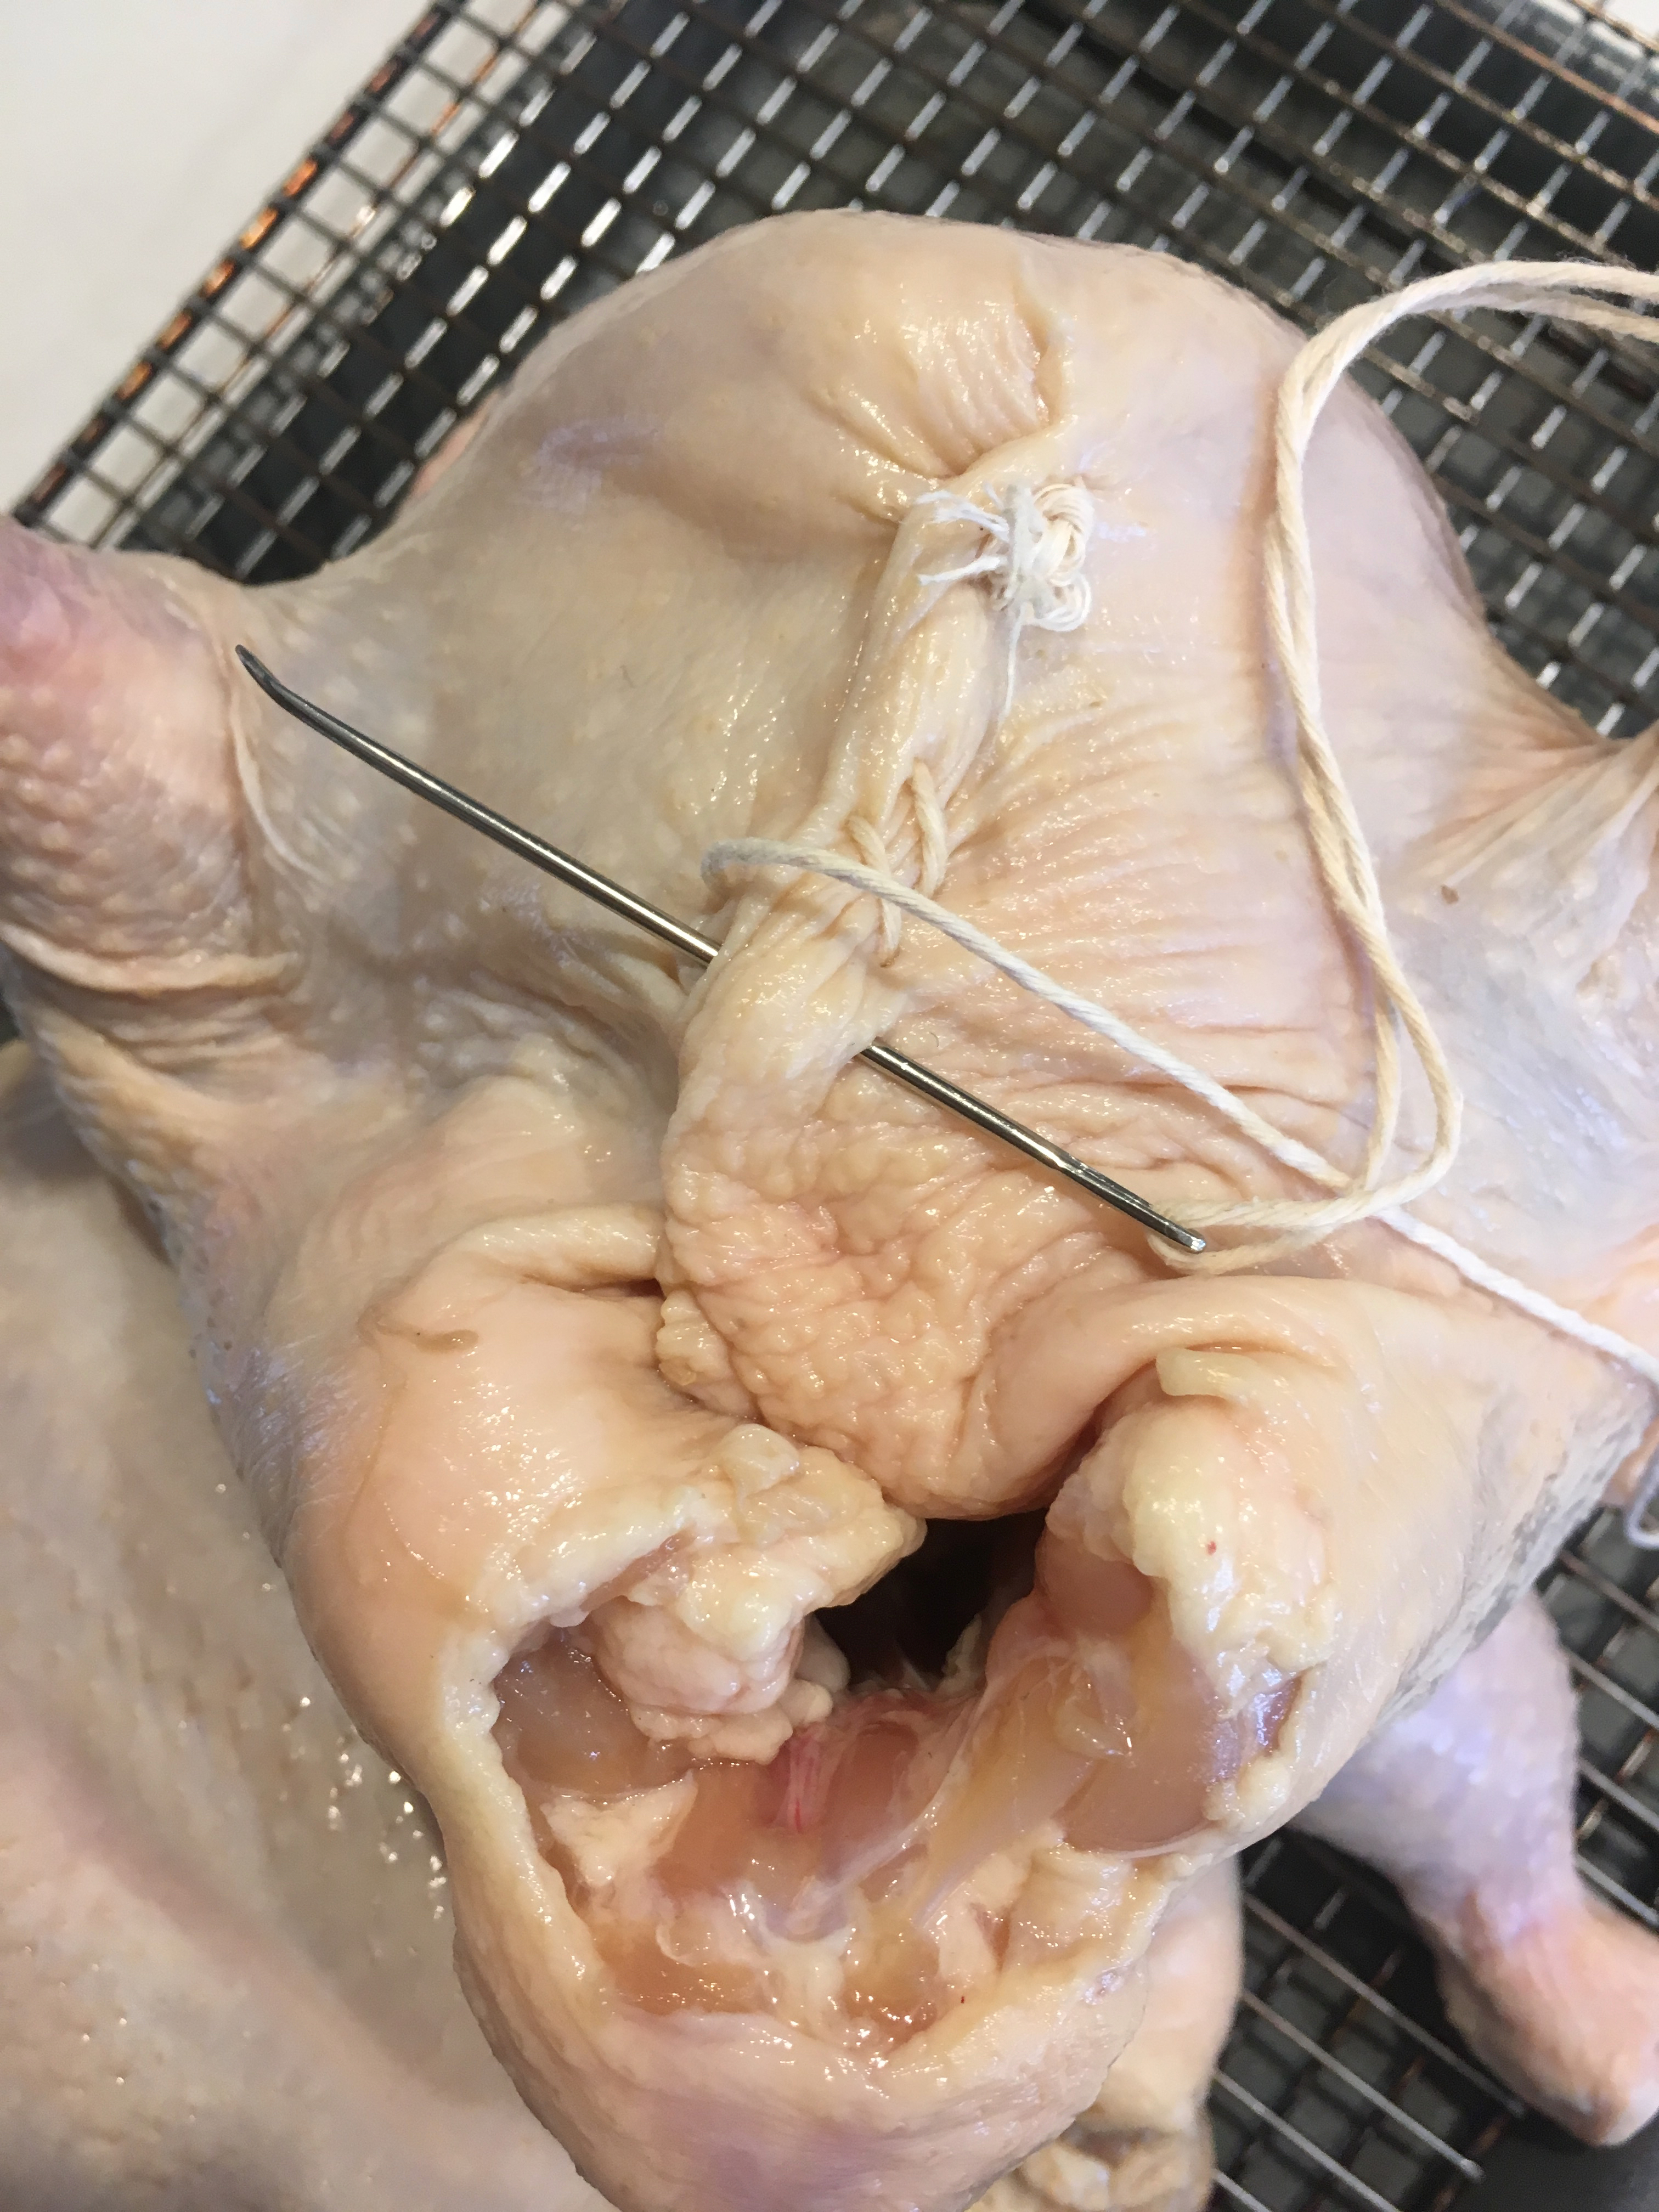
\includegraphics[width=0.25\textwidth]{\imageDir/\fileName/IMG_3214.jpg} &
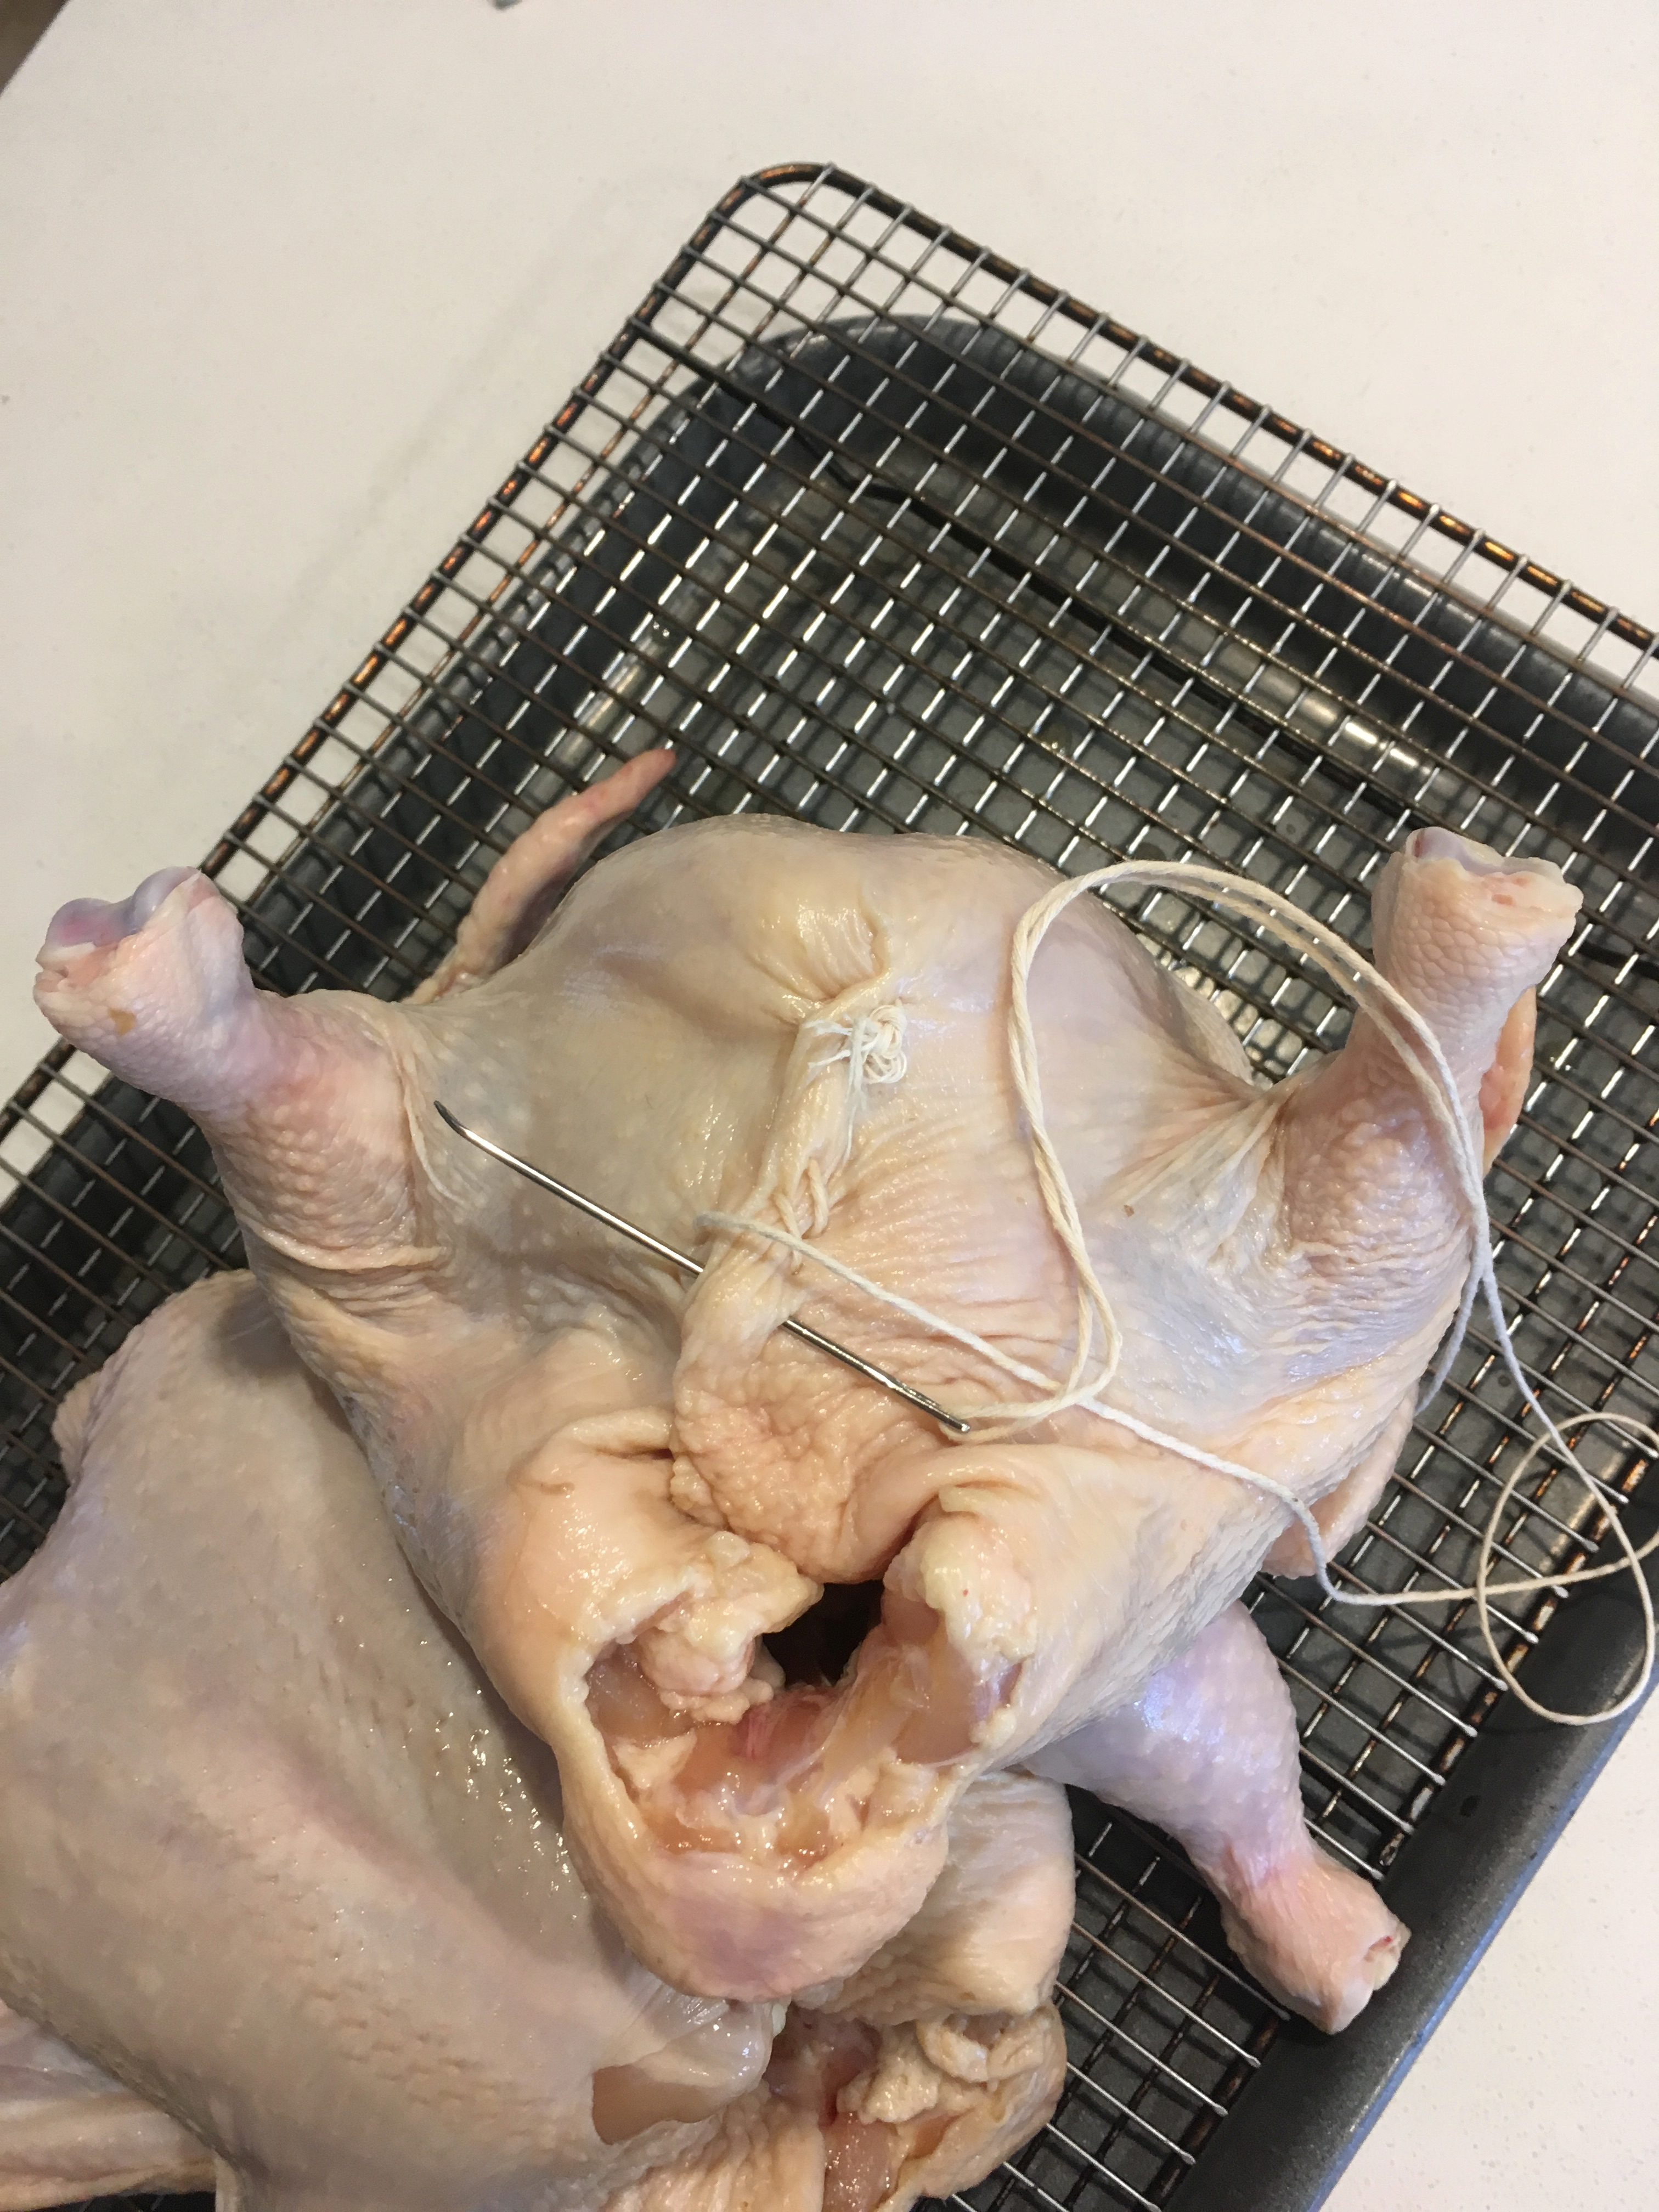
\includegraphics[width=0.25\textwidth]{\imageDir/\fileName/IMG_3216.jpg} \\
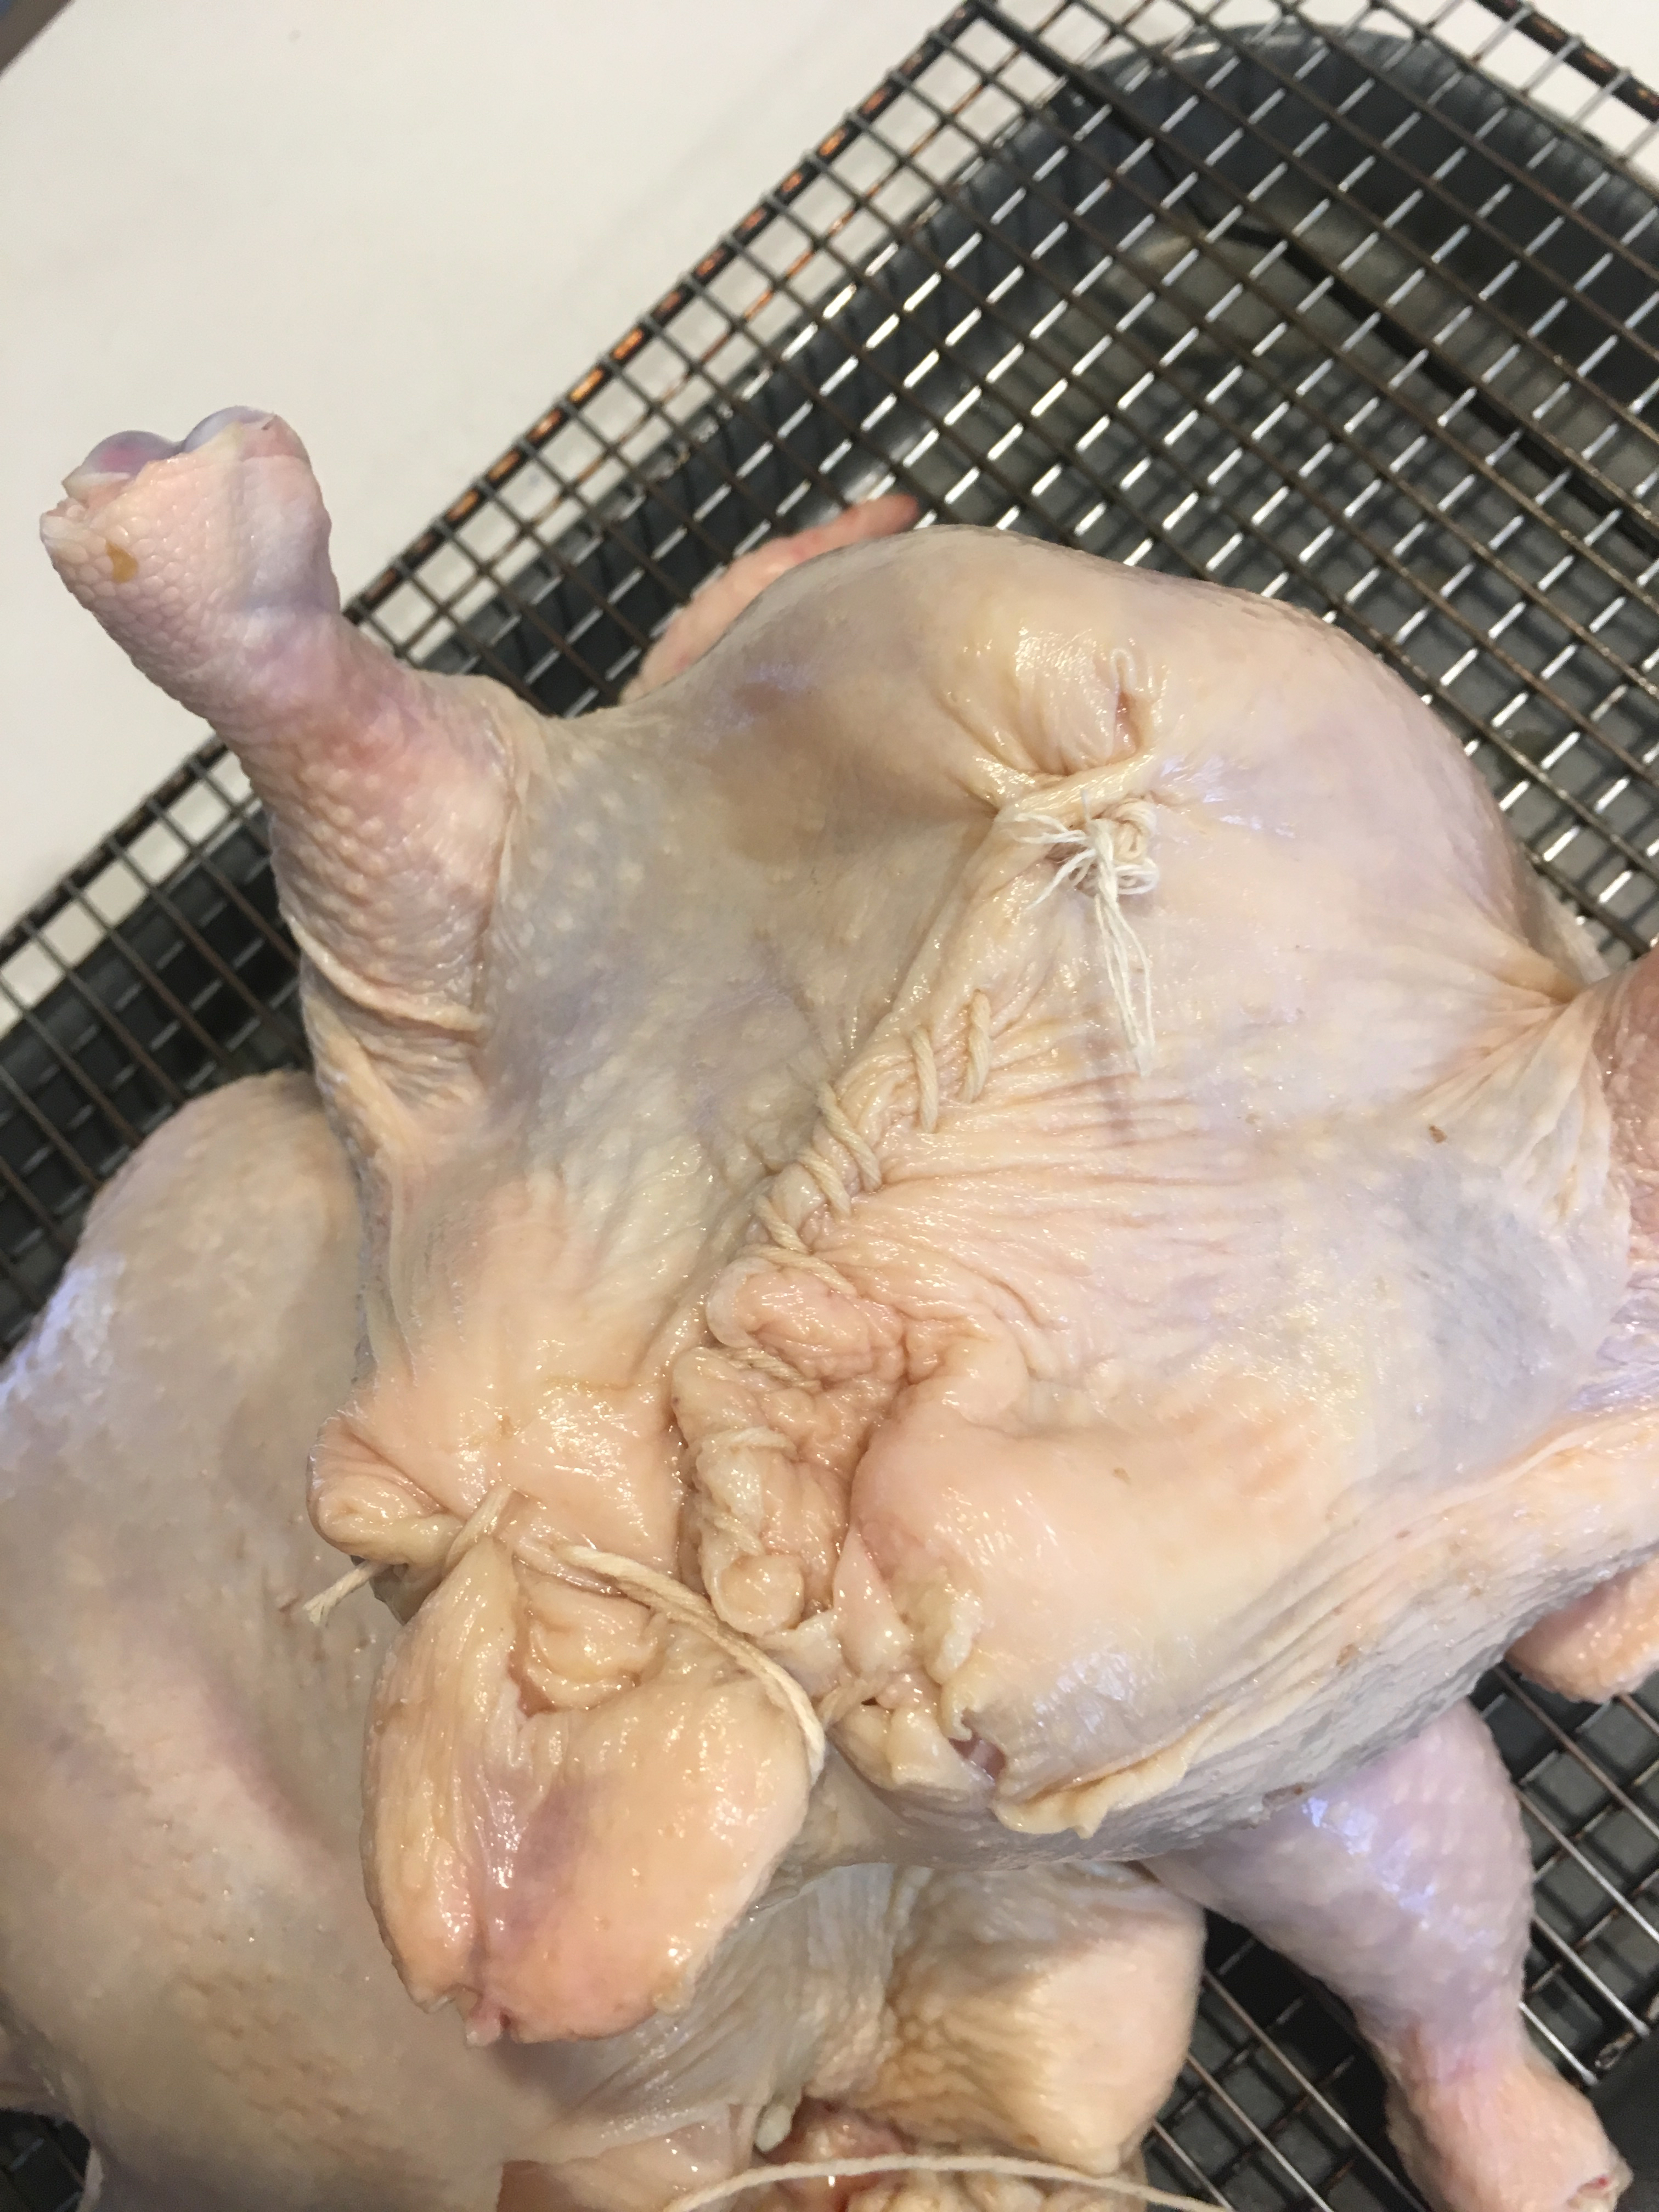
\includegraphics[width=0.25\textwidth]{\imageDir/\fileName/IMG_3217.jpg} &
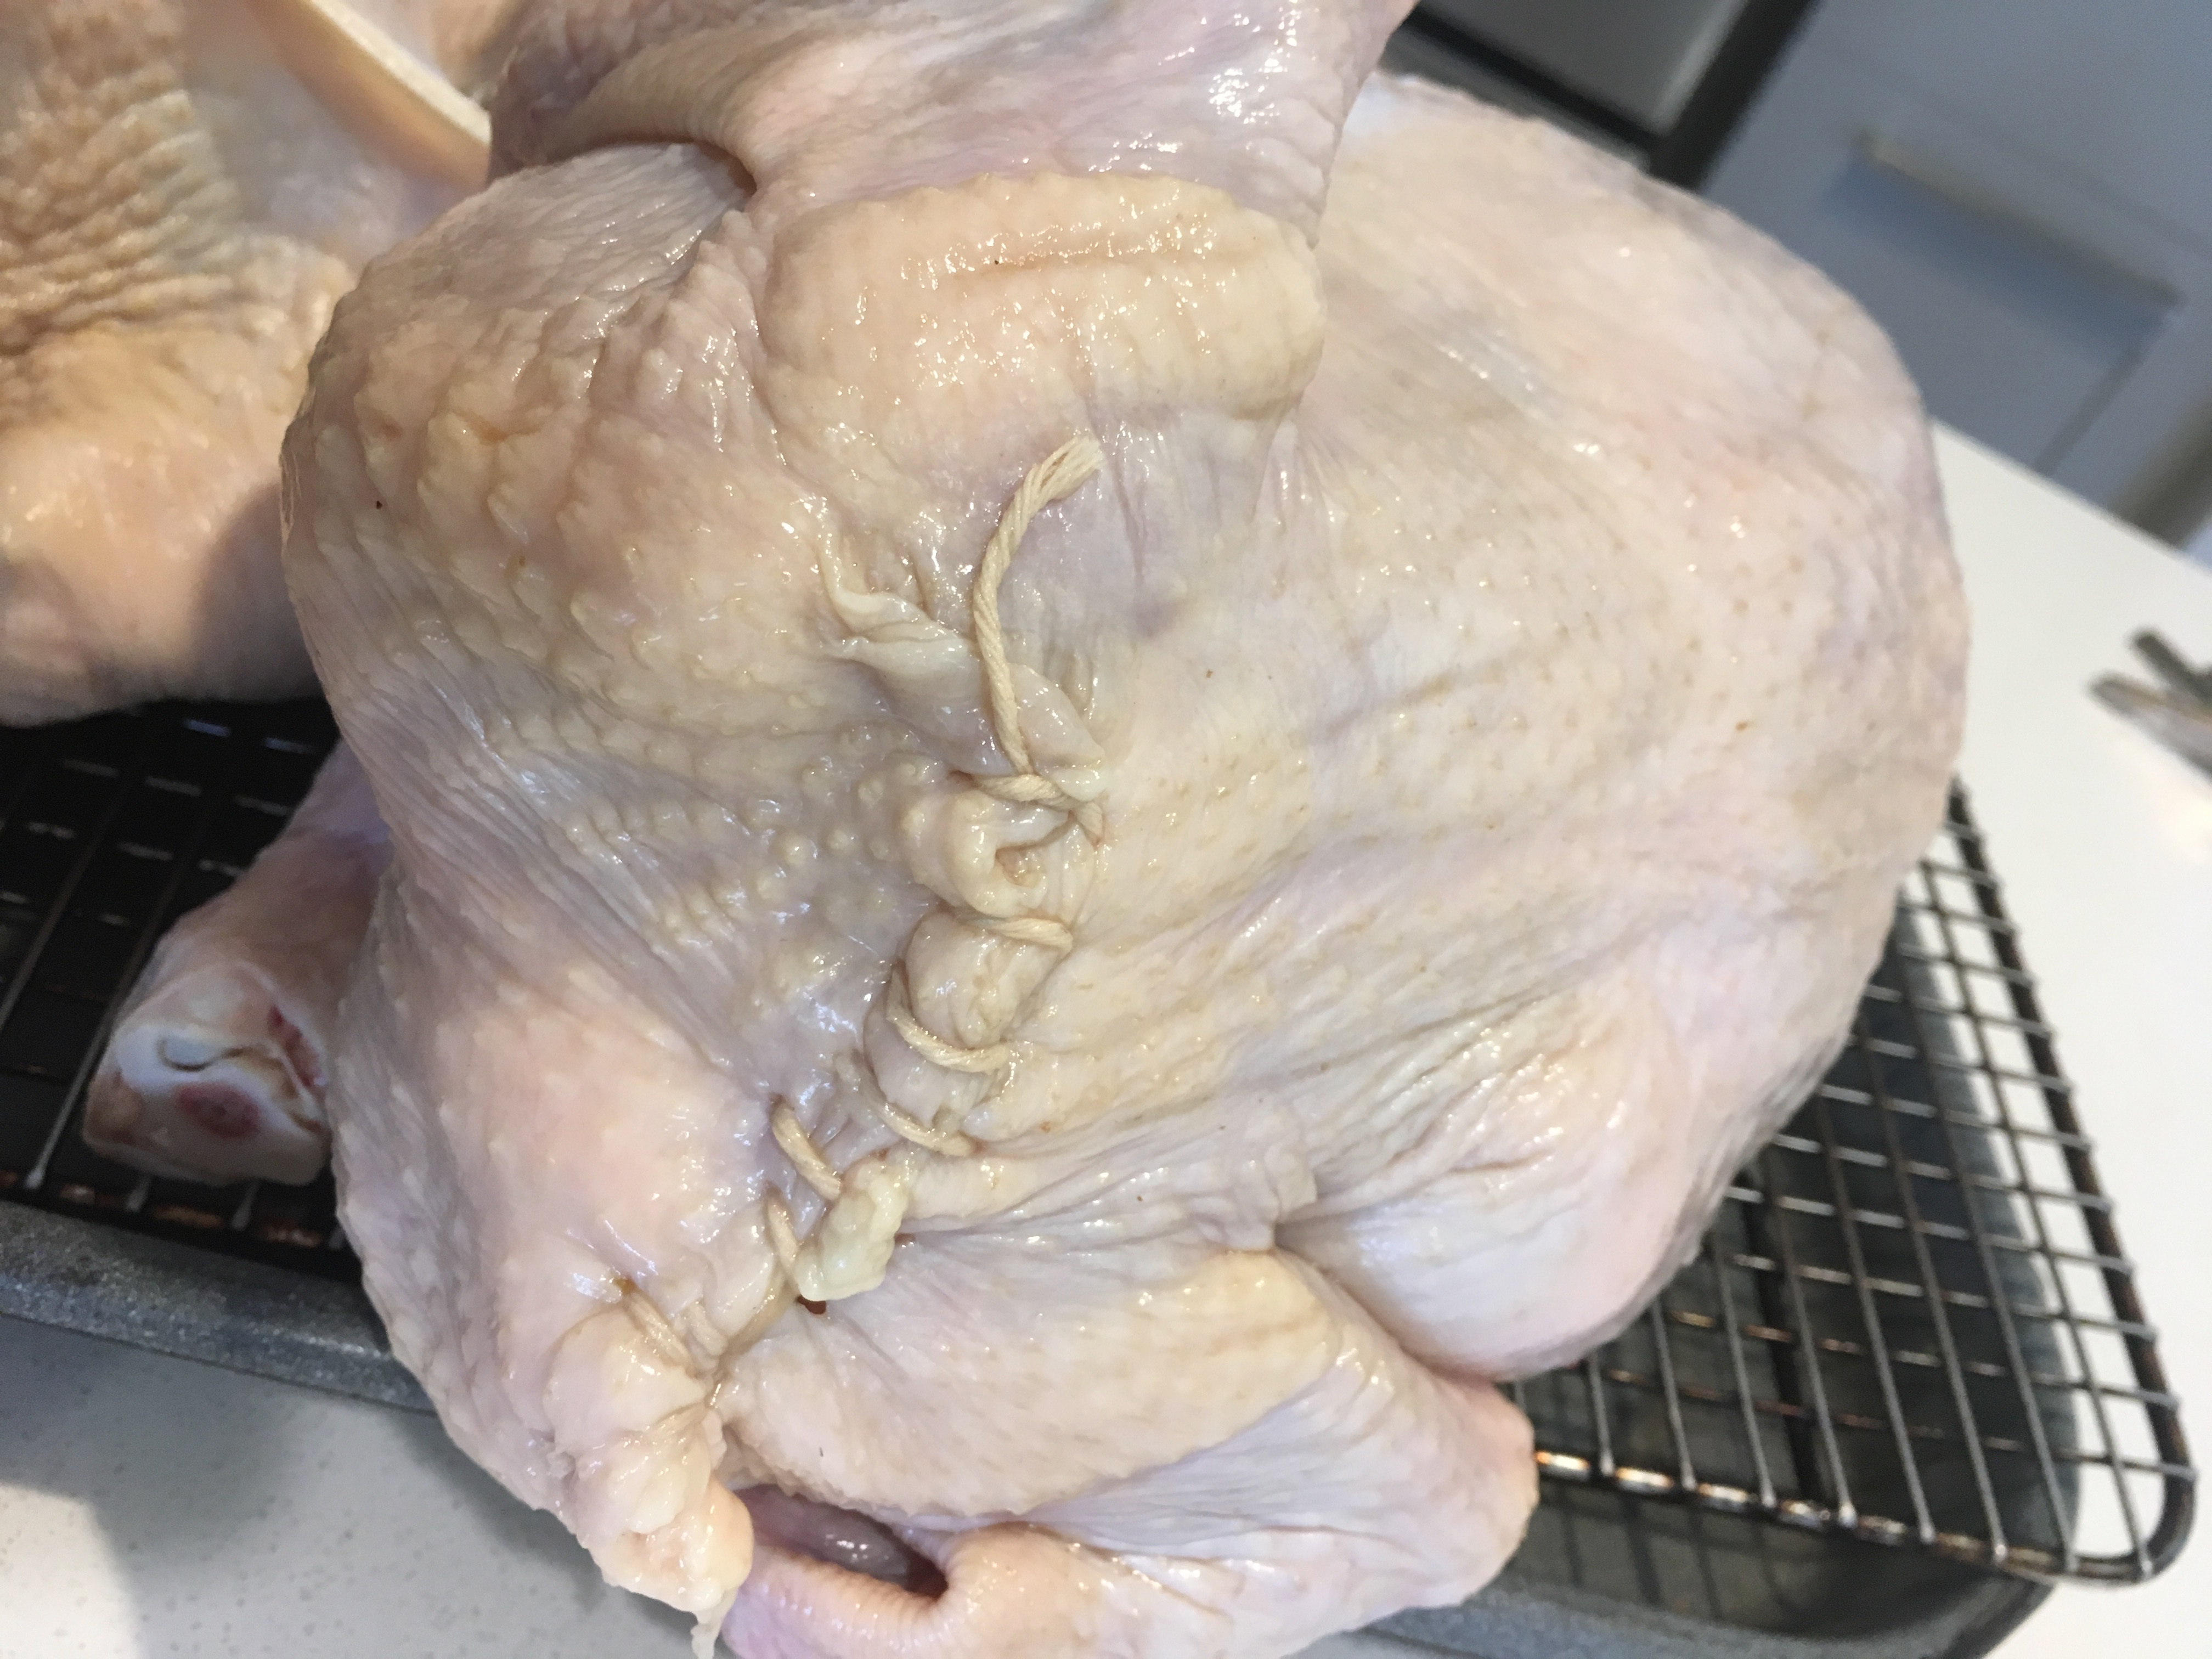
\includegraphics[width=0.25\textwidth]{\imageDir/\fileName/IMG_3218.jpg} &
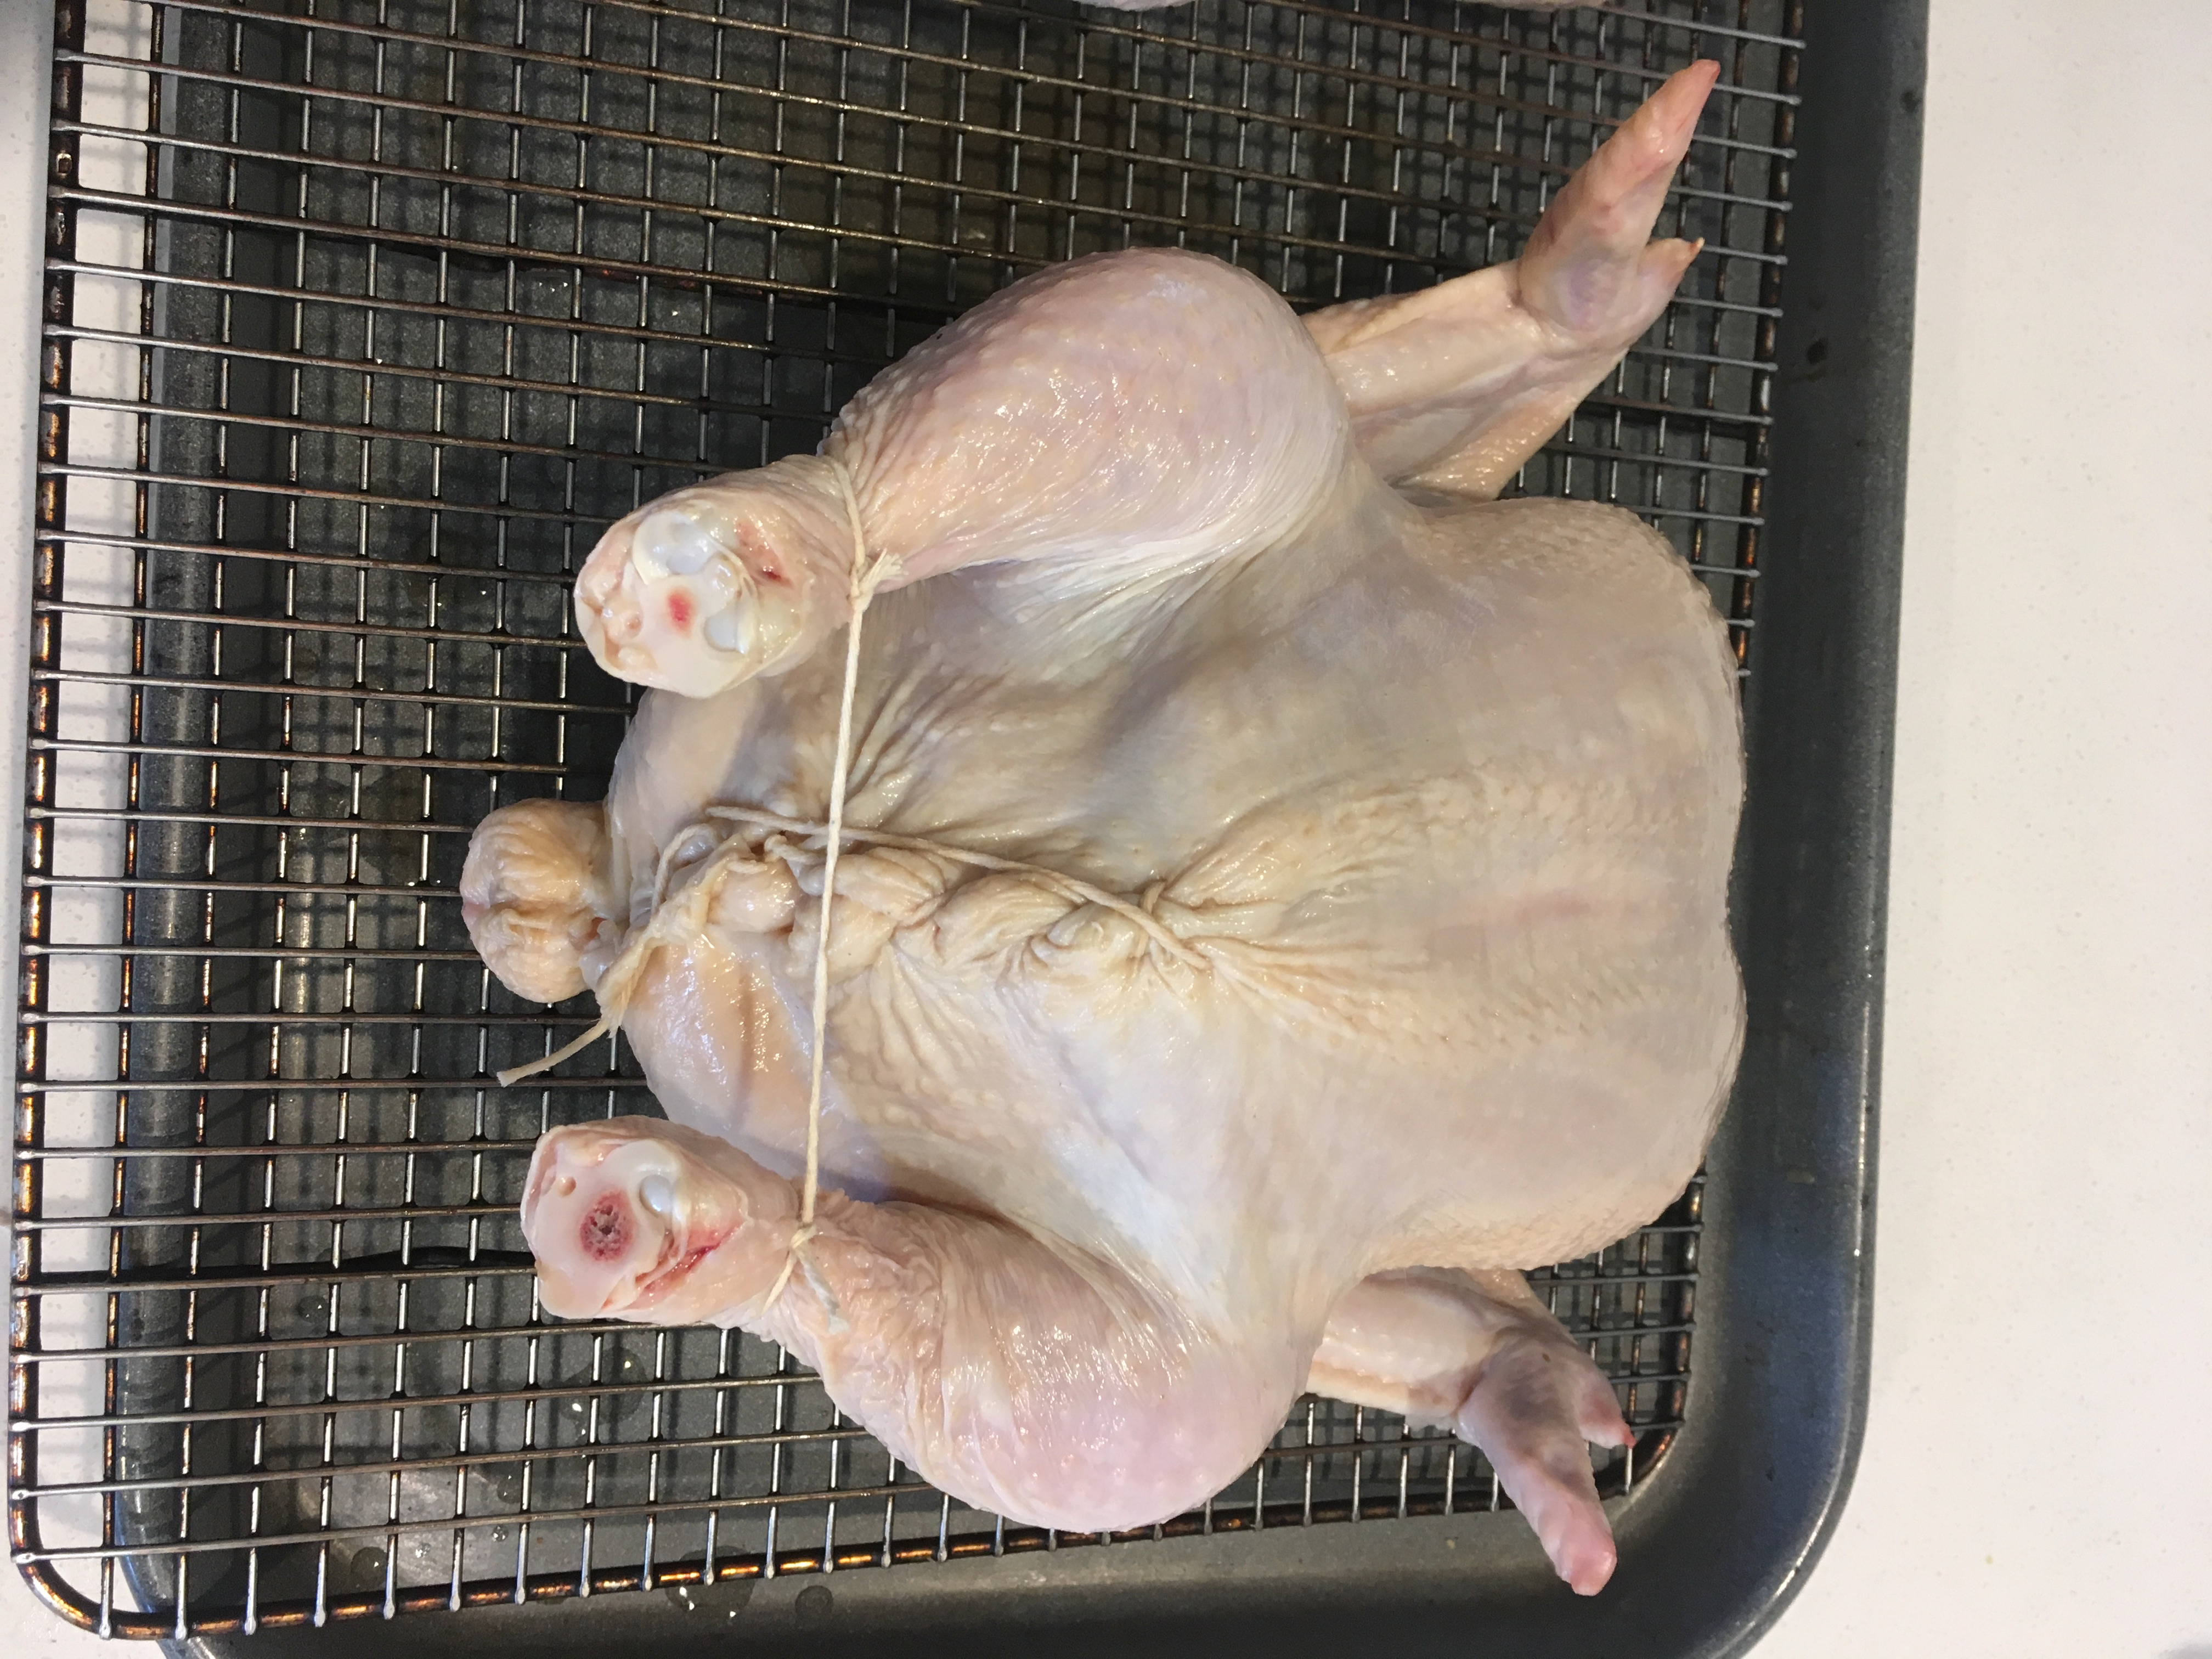
\includegraphics[width=0.25\textwidth]{\imageDir/\fileName/IMG_3219.jpg} \\
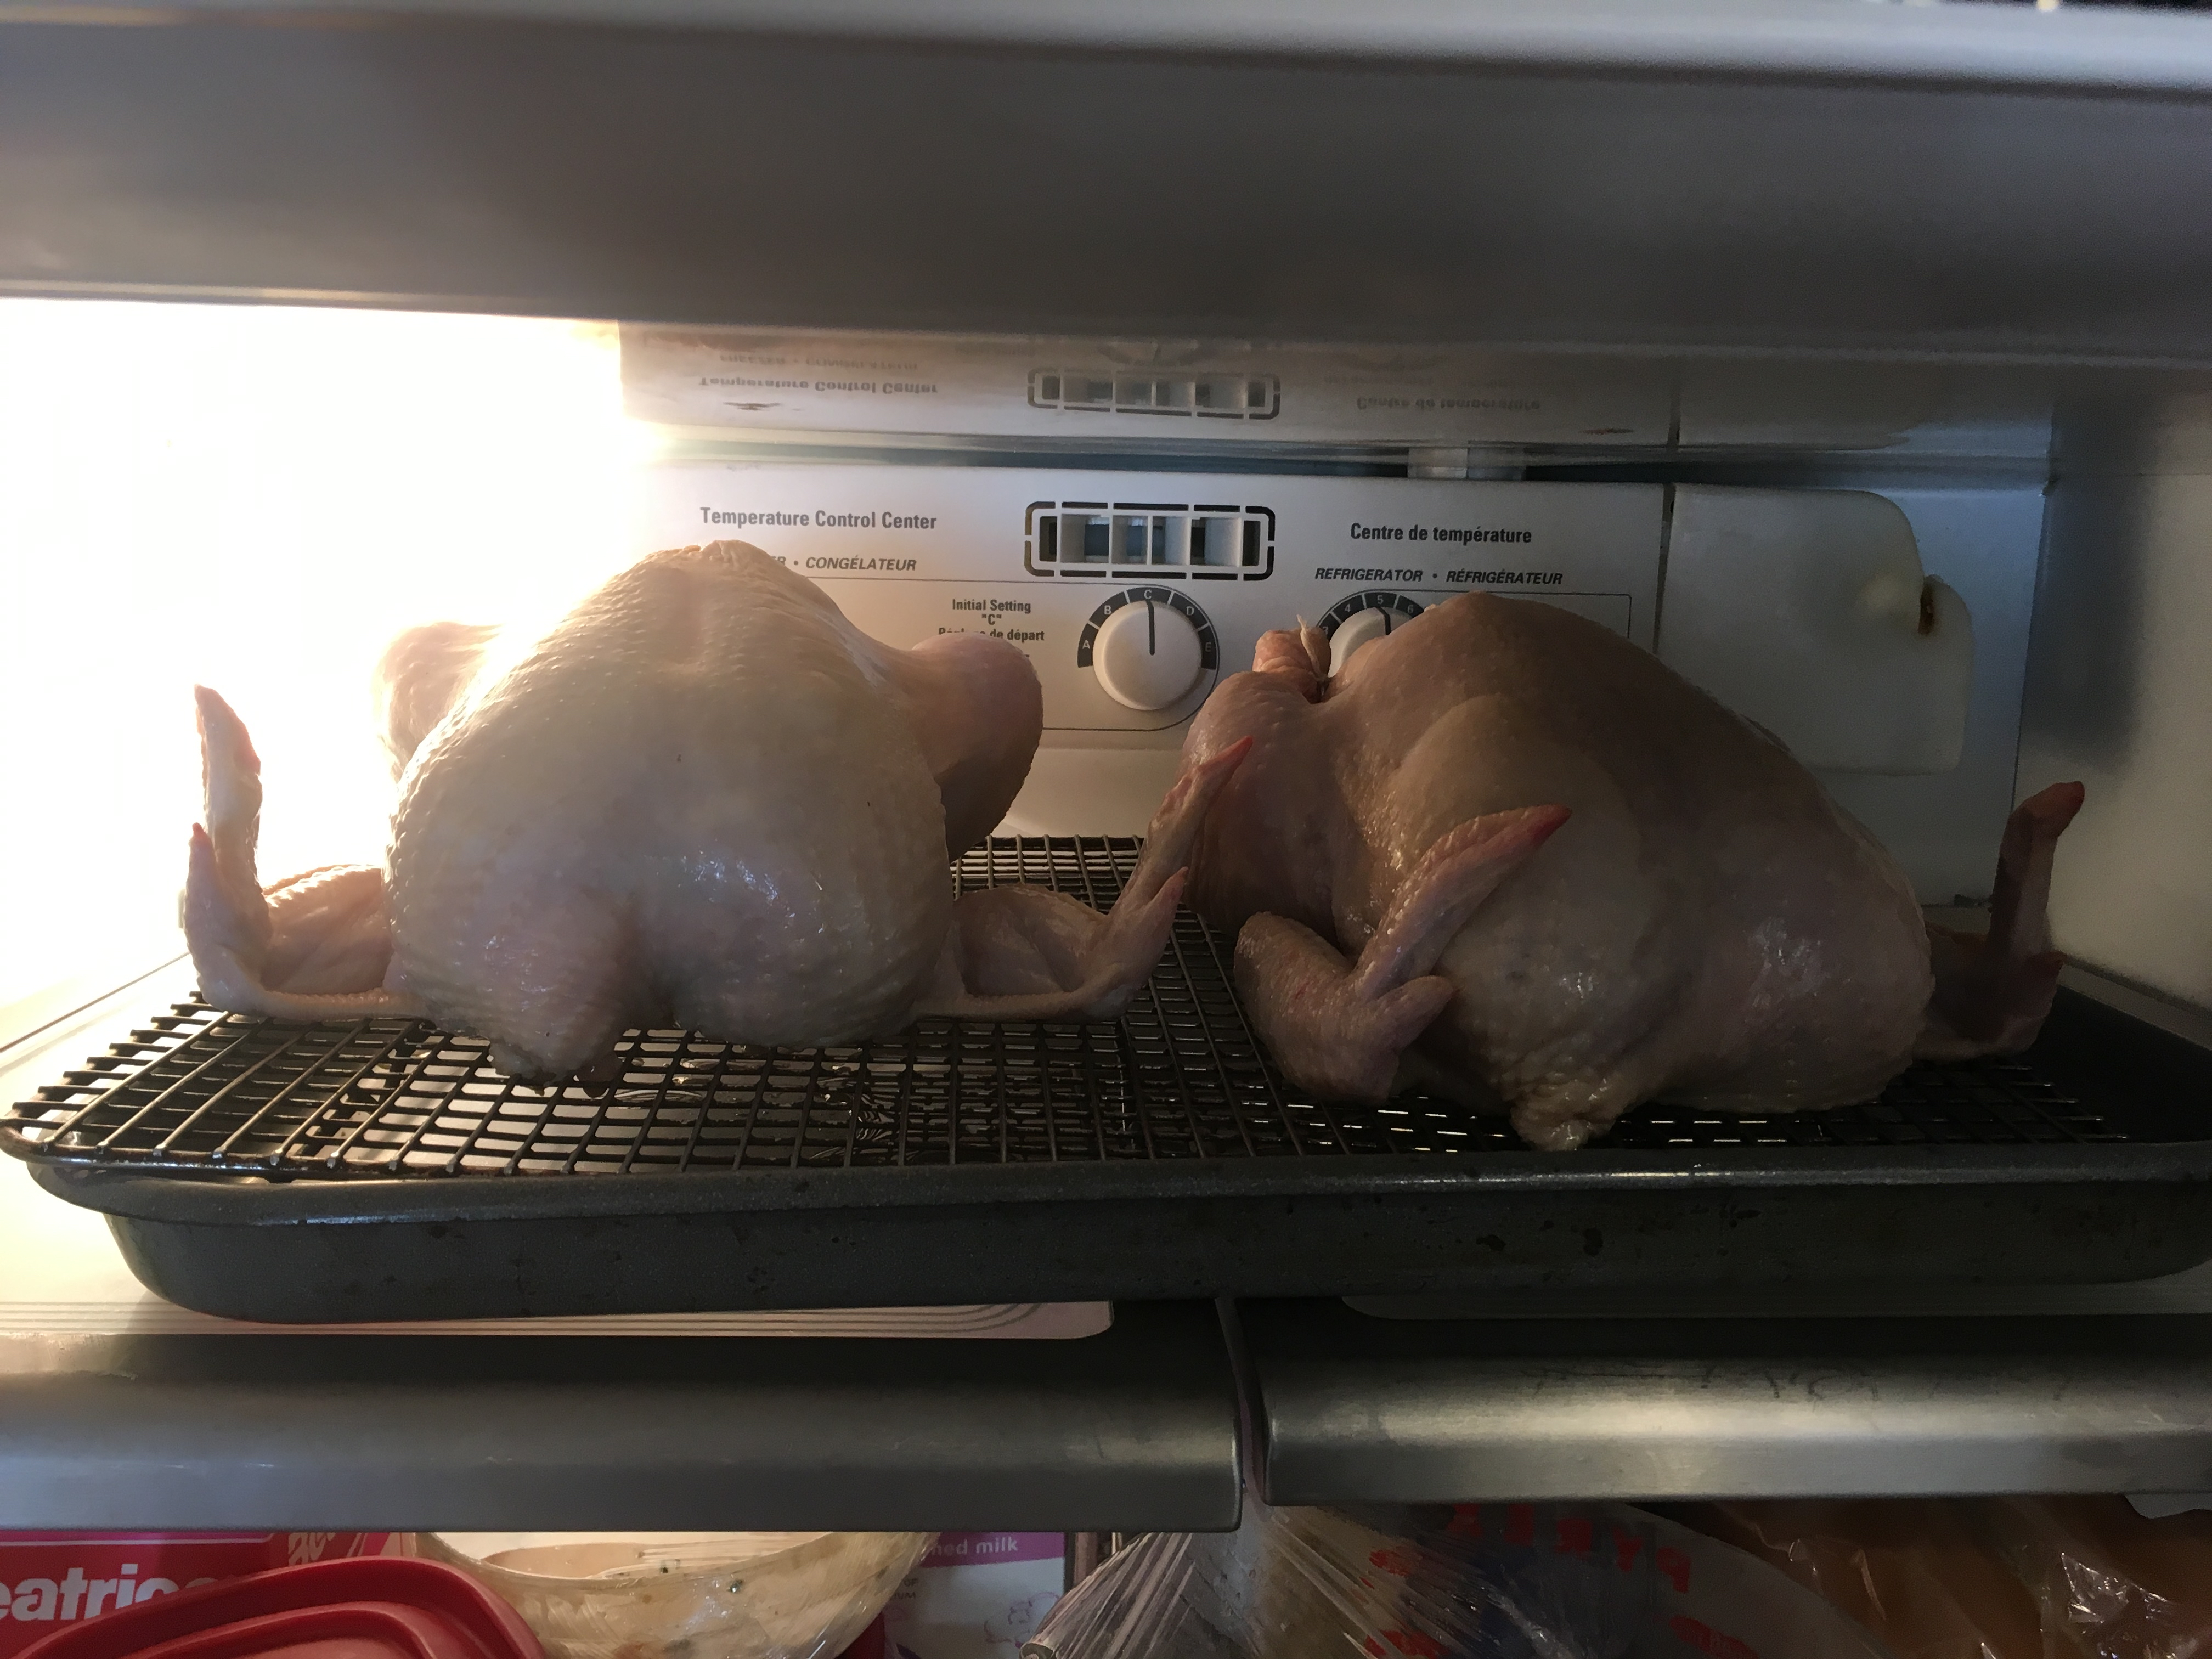
\includegraphics[width=0.25\textwidth]{\imageDir/\fileName/IMG_3220.jpg} &
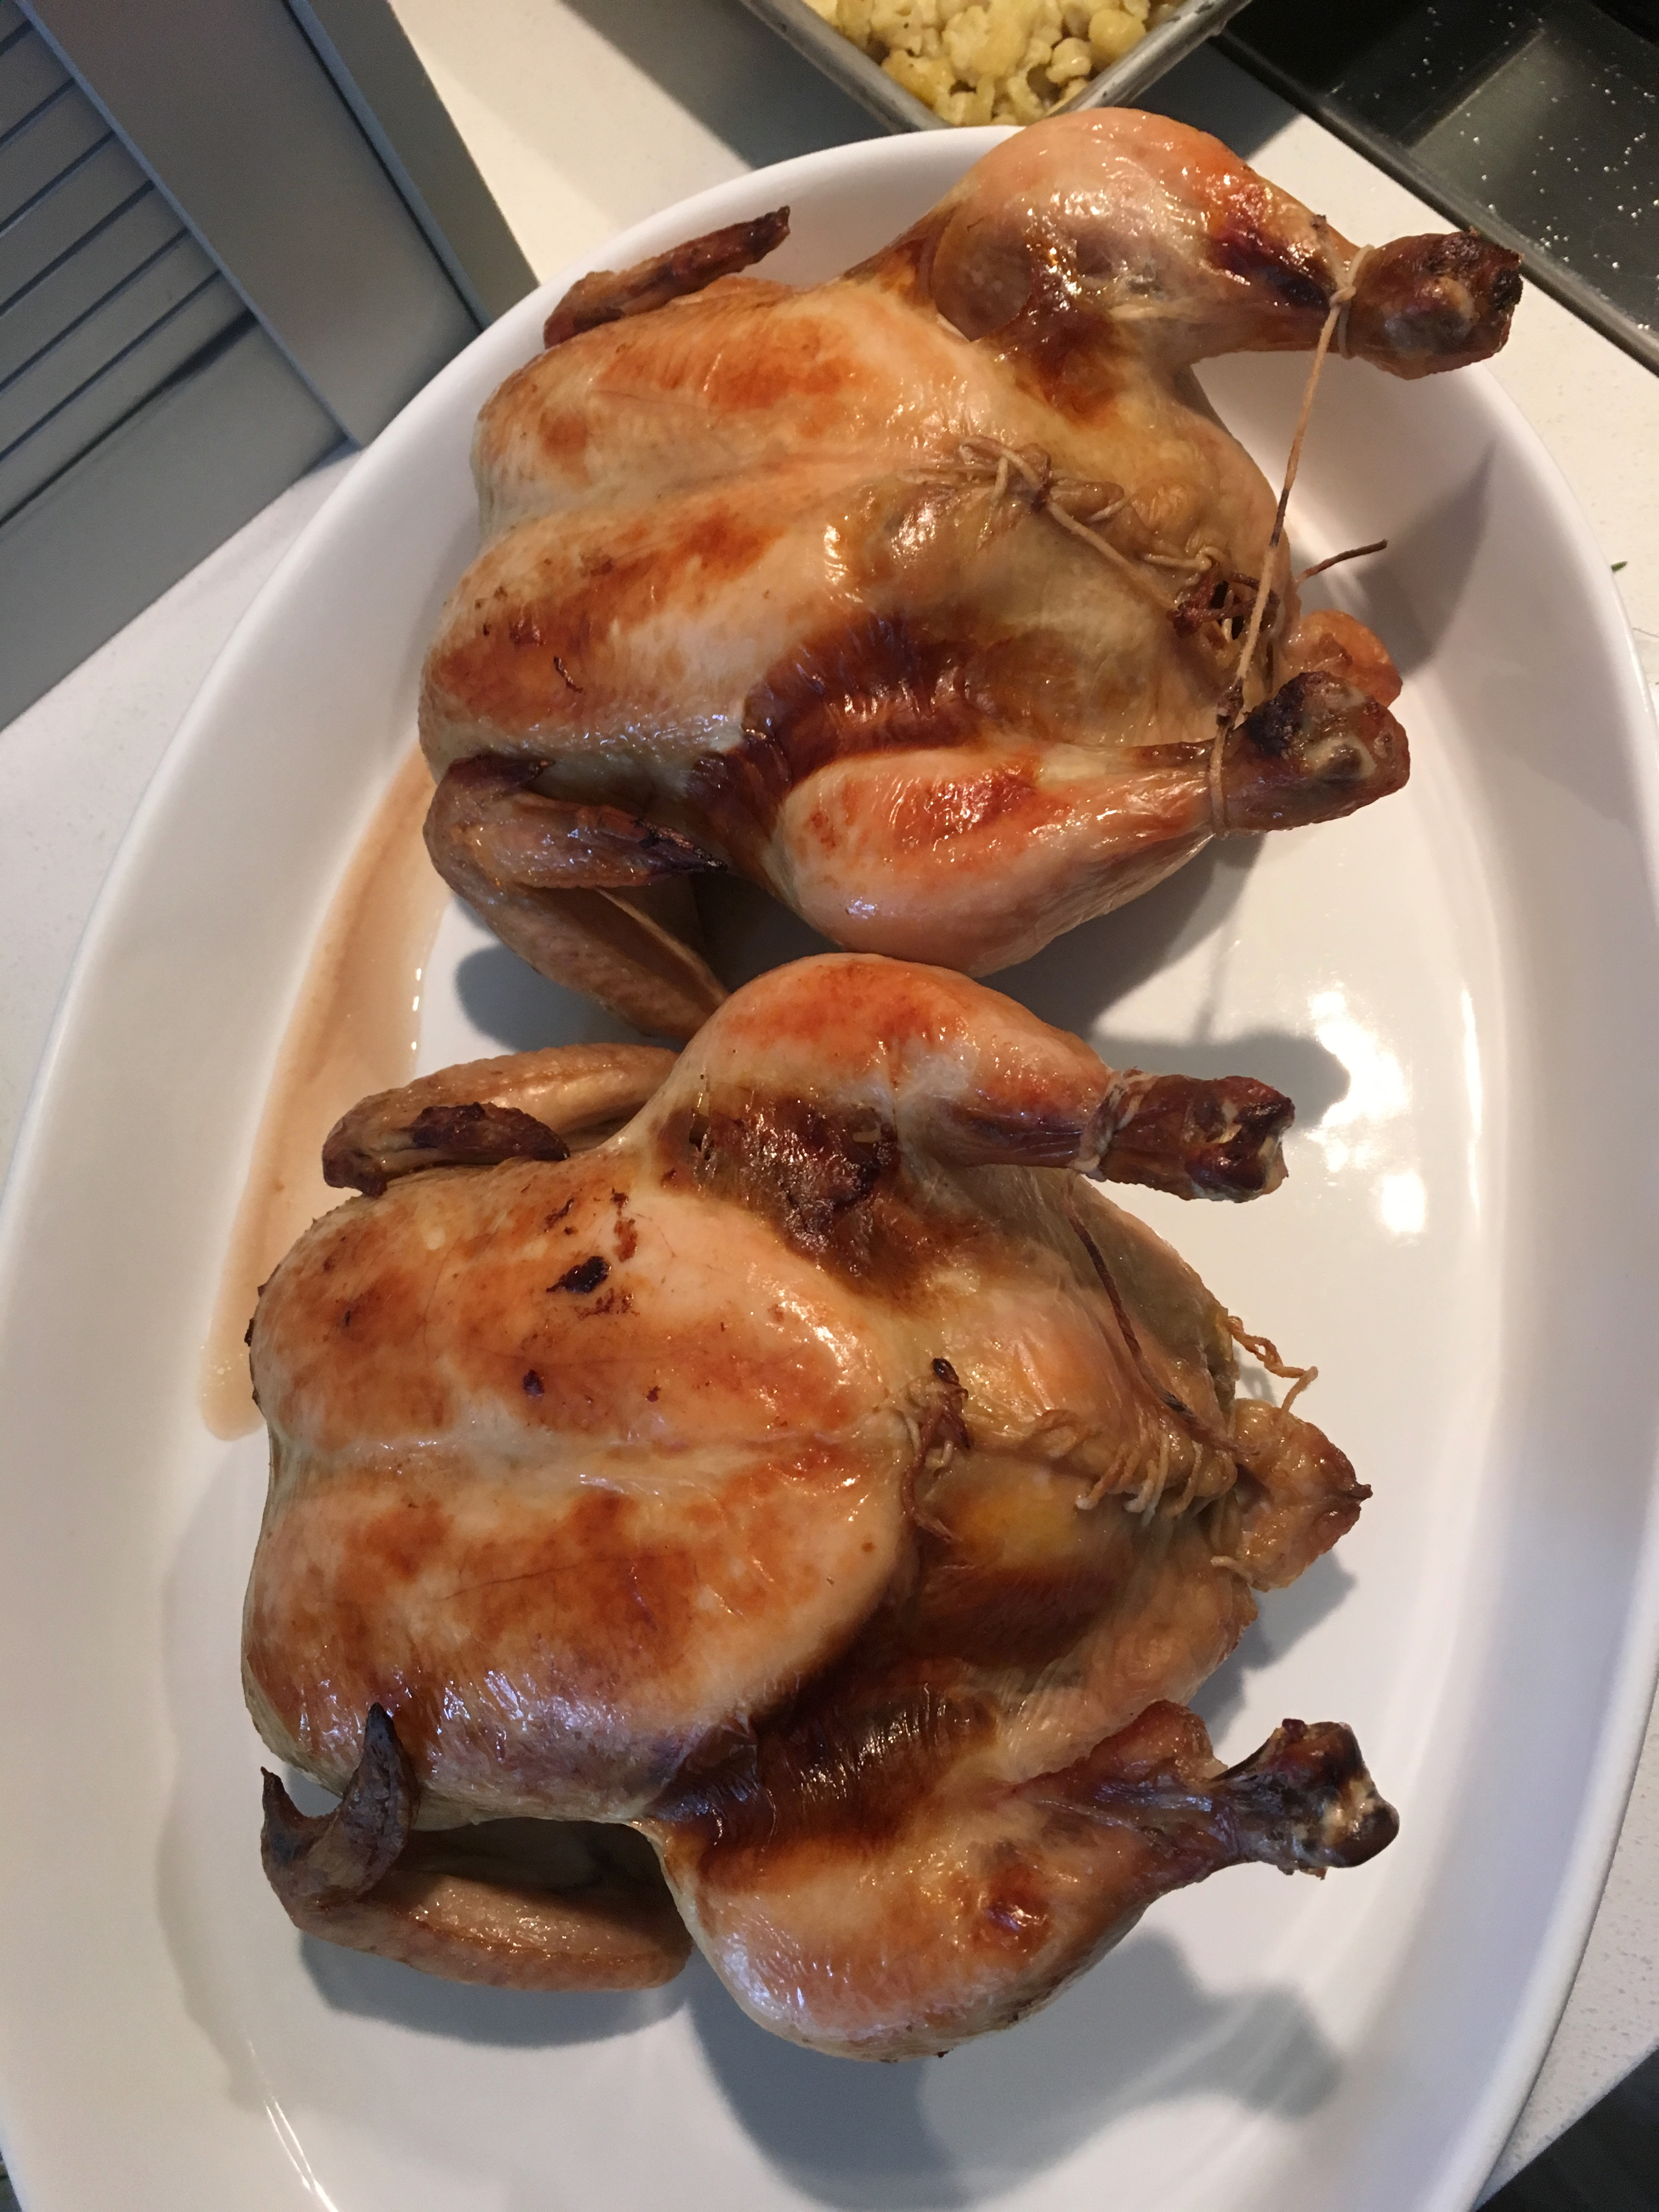
\includegraphics[width=0.25\textwidth]{\imageDir/\fileName/IMG_3228.jpg} \\
\end{tabular}
\end{table}


\end{document}



